\documentclass[journal]{IEEEtran}
% Avoid malformed compressed object streams in some PDF readers.
\ifdefined\pdfobjcompresslevel
  \pdfobjcompresslevel=0
\fi
\usepackage{amsmath,amsfonts}
\usepackage{algpseudocode}
\usepackage{algorithm}
\usepackage{array}
\usepackage{booktabs}
\usepackage[caption=false,font=normalsize,labelfont=sf,textfont=sf]{subfig}
\usepackage{multirow}
\usepackage{siunitx}
\usepackage{textcomp}
\usepackage{stfloats}
\usepackage{bm}
\usepackage{threeparttable}
\usepackage{url}
\usepackage{verbatim}
\usepackage{graphicx}
\usepackage{tikz}
\usepackage{cite}
\usetikzlibrary{positioning,calc}
\hyphenation{op-tical net-works semi-conduc-tor IEEE-Xplore}
\usepackage{tikz}
\usepackage{pgfplots}
\pgfplotsset{compat=1.18}
\usepackage[american]{circuitikz}
\usetikzlibrary{calc, positioning, arrows.meta}
\newcommand{\stdplot}[4][]{%
  \begin{tikzpicture}
    \node[inner sep=0] (stdplotimage) {\includegraphics[
      #1,trim=12pt 14pt 0pt 0pt,clip]{#2}};
    \fill[white] (stdplotimage.south west)
      rectangle ([xshift=1.5mm]stdplotimage.north west);
    \node[inner sep=0.4pt,font=\footnotesize]
      at ([yshift=-2.2mm]stdplotimage.south) {#3};
    \node[inner sep=0.4pt,font=\footnotesize,
          minimum width=0.40\linewidth,rotate=90]
      at ([xshift=-3.2mm]stdplotimage.west) {#4};
  \end{tikzpicture}%
}
\newcommand{\stdxplot}[3][]{%
  \begin{tikzpicture}
    \node[inner sep=0] (stdxplotimage) {\includegraphics[
      #1,trim=0pt 14pt 0pt 0pt,clip]{#2}};
    \node[inner sep=0.4pt,font=\footnotesize]
      at ([yshift=-2.2mm]stdxplotimage.south) {#3};
  \end{tikzpicture}%
}
\newcommand{\stdthreephaseplot}[2][]{%
  \begin{tikzpicture}
    \node[inner sep=0] (stdthreeimage) {\includegraphics[
      #1,trim=12pt 14pt 0pt 0pt,clip]{#2}};
    \fill[white] (stdthreeimage.south west)
      rectangle ([xshift=1.5mm]stdthreeimage.north west);
    \node[inner sep=0.4pt,font=\footnotesize]
      at ([yshift=-2.2mm]stdthreeimage.south) {Time, $t$ [h]};
    \node[inner sep=0.3pt,font=\scriptsize,rotate=90]
      at ($([xshift=-3mm]stdthreeimage.south west)!0.83!
            ([xshift=-3mm]stdthreeimage.north west)$) {$\Delta V_A$ [pu]};
    \node[inner sep=0.3pt,font=\scriptsize,rotate=90]
      at ($([xshift=-3mm]stdthreeimage.south west)!0.50!
            ([xshift=-3mm]stdthreeimage.north west)$) {$\Delta V_B$ [pu]};
    \node[inner sep=0.3pt,font=\scriptsize,rotate=90]
      at ($([xshift=-3mm]stdthreeimage.south west)!0.17!
            ([xshift=-3mm]stdthreeimage.north west)$) {$\Delta V_C$ [pu]};
  \end{tikzpicture}%
}
\hbadness=10000
\vbadness=10000
\hfuzz=8pt
\newcommand{\compactpartial}[2]{%
    \compactpartialaux#1\compactstop#2\compactstop}
\def\compactpartialaux\partial#1\compactstop\partial#2\compactstop{%
    \partial_{#2}#1}
% updated with editorial comments 8/9/2021

\begin{document}
\title{Optimal Tuning of Static Var Compensators for\\ Power Quality Enhancement in Distribution Systems: An Approach \\ using the Three-Phase Harmonic Current Injection Method}
\author{Robert W. da Silva, Igor D. de Melo, Leticia L. S. de Sousa
%\thanks{Manuscript created October, 2020; This work was developed by the IEEE Publication Technology Department. This work is distributed under the \LaTeX \ Project Public License (LPPL) ( http://www.latex-project.org/ ) version 1.3. A copy of the LPPL, version 1.3, is included in the base \LaTeX \ documentation of all distributions of \LaTeX \ released 2003/12/01 or later. The opinions expressed here are entirely that of the author. No warranty is expressed or implied. User assumes all risk.}
}

\markboth{Journal of \LaTeX\ Class Files,~Vol.~18, No.~9, September~2020}%
{How to Use the IEEEtran \LaTeX \ Templates}

\maketitle

\begin{abstract}
This work proposes a nonlinear optimization methodology for controlling Static Var Compensators (SVCs) in distribution systems. The objective function combines the minimization of voltage deviation, negative-sequence voltage and phase unbalance indices. The formulation is based on the Harmonic Three-Phase Current Injection Method (HTPCIM), representing each compensator through topology-dependent harmonic current injection equations and associated control variables. The numerical implementation enables independent adjustment of the firing angle of each three-phase branch, allowing branch-specific reactive power compensation according to network operating conditions. In addition to voltage magnitudes and total harmonic distortion (THD) constraints, the formulation incorporates a voltage unbalance factor (VUF) constraint, evaluated using the positive- and negative-sequence voltage components. The proposed methodology is evaluated using IEEE benchmark test feeders under balanced and unbalanced loading conditions. Numerical results demonstrate that optimized SVC control increases the loading capability of controlled buses and improves voltage profiles. Furthermore, under suitable operating conditions, the proposed strategy reduces phase unbalance while maintaining voltage and THD limits. The results highlight the potential of the proposed optimization framework as a flexible solution for coordinating SVC operation in distribution networks subject to varying loading conditions. By simultaneously addressing voltage regulation, harmonic distortion, and phase unbalance, the methodology provides a comprehensive approach to improving power quality and enhancing the operational performance of distribution systems.
\end{abstract}

\begin{IEEEkeywords}
 Power Quality, Harmonic analysis, Static Var Compensators, Optimization, Distribution Systems.
\end{IEEEkeywords}


\section{Introduction}
 \IEEEPARstart{D}{istribution} systems operate under increasingly complex technical conditions due to the combined effects of load variability, phase unbalance, nonlinear consumer devices, and limited voltage support along radial feeders. In practical networks, these characteristics may lead to unequal phase loading, harmonic distortion, voltage drops at remote buses, and reduced operating margins, particularly in long feeders and under loading conditions above nominal levels~\cite{loji2023operational}. From the operational viewpoint, these challenges are further intensified by the ongoing transformation of distribution grids, particularly the increasing penetration of distributed generation and the rapid growth of electric-vehicle charging demand~\cite{nasir2024hosting,ghaffari2025planning}. In parallel, artificial-intelligence techniques are increasingly being investigated for the detection, classification, prediction, and mitigation of power-quality disturbances in distribution systems~\cite{dehaghani2025ai}.

Within this scenario, power-electronics-based equipment has become increasingly relevant in distribution systems because it enables fast and flexible actions for voltage regulation, reactive power compensation, power-flow support, and overall power-quality improvement~\cite{Stanelyte2020VoltVar}. This is particularly important because voltage drops at the end of feeders and phase unbalance remain persistent operational challenges, while conventional utility assets often provide limited dynamic controllability. Consequently, distribution utilities must deal with networks whose monitoring and control capabilities may be insufficient for the real-time mitigation of local disturbances and phase-dependent voltage deviations, especially in low-observability feeders~\cite{Yadav2023DSSE}. Among the available solutions, Static Var Compensators (SVCs), based on thyristor-controlled reactive power devices, represent an attractive alternative for providing dynamic reactive power compensation and voltage regulation~\cite{Stanelyte2020VoltVar,Liu2020SVCUnbalance}. Their controllable operating characteristics also make them suitable for optimization-based control strategies aimed at improving the operating conditions of distribution networks.

However, voltage regulation alone may be insufficient when the problem is considered from a broader power-quality perspective. Thyristor-based compensators are nonlinear devices that may introduce harmonic components into the network. Characteristic low-order harmonics, such as the 5th, 7th, 11th, and 13th, are commonly associated with these devices, depending on their circuit configuration and filtering conditions~\cite{Kraimia2021SVCHarmonics,Zheng2021SVCHarmonicFailure}. Furthermore, the interaction between compensator components and network impedances may create resonance conditions capable of amplifying voltage distortion, increasing total harmonic distortion (THD), and contributing to overvoltage phenomena~\cite{Farzin2022CapacitorResonance}. Phase unbalance represents an additional concern because it may increase neutral currents, intensify losses and thermal stresses in conductors and equipment, and deteriorate the operating conditions of sensitive loads and rotating machines~\cite{Liu2020SVCUnbalance}. These aspects indicate that reactive power compensation should be addressed through control strategies that simultaneously consider voltage regulation, harmonic distortion, and phase unbalance.

In this context, this paper proposes a nonlinear optimization methodology for SVC control based on the Harmonic Three-Phase Current Injection Method (HTPCIM)~\cite{variz2006three}. HTPCIM extends the Three-Phase Current Injection Method (TCIM), originally developed for fundamental-frequency unbalanced power-flow calculations~\cite{garcia2000three}, to the harmonic domain~\cite{variz2006three}. By adopting a current-injection representation, the proposed formulation provides flexibility in modeling SVCs with different electrical configurations and operating characteristics. Each compensator is represented through its corresponding topology-dependent harmonic current injection equations, control variables, and operating constraints, without restricting the optimization framework to a particular internal arrangement or connection topology. This representation also allows the control variables to be defined according to the physical characteristics of the device, including the independent adjustment of the firing angles of individual three-phase branches when applicable.

The main contribution of this work is the development of an integrated nonlinear optimization framework that coordinates SVC operation while explicitly accounting for the interaction between voltage regulation, phase unbalance, and harmonic distortion. Unlike approaches focused exclusively on reactive power compensation or voltage profile improvement, the proposed objective function combines indices associated with voltage deviation, negative-sequence voltage, and phase unbalance. In addition, voltage magnitude, THD, and voltage unbalance factor (VUF) limits are explicitly incorporated into the optimization problem, with the latter evaluated from the positive- and negative-sequence voltage components. The formulation therefore enables the optimization process to improve network operating conditions without disregarding the power-quality restrictions imposed on the system. The numerical implementation further allows independent control of the firing angle of each SVC branch, providing additional flexibility in the distribution of reactive power compensation according to the network operating condition.

The proposed methodology is evaluated using the IEEE test feeders under balanced and unbalanced loading conditions. The numerical results are used to assess its capability to increase the loading capability of controlled buses, improve voltage profiles, and mitigate phase unbalance while maintaining harmonic distortion within the prescribed limits. Overall, this work provides a flexible optimization framework for SVC control that integrates fundamental-frequency operating requirements and harmonic-domain constraints, contributing to improved power quality and enhanced operational performance in distribution systems.



The remainder of this paper is organized as follows. Section II describes the SVC modeling based on HTPCIM, including its harmonic current injection equations and control variables. Then, the mathematical formulation of the proposed SVC control methodology is presented, including the objective function, operating constraints, and nonlinear optimization model. Section III presents the test system and numerical results under balanced and unbalanced loading conditions. Finally, Section IV presents the main conclusions of this work.

\section{The Proposed Methodology}
\label{sec:methodology}



% -------------------------------------------------------------------------
\subsection{Static Var Compensator Model}
\label{subsec:svc_rating}



A typical SVC configuration is illustrated in
Fig.~\ref{fig:delta_fc_tcr_svc}. It consists of a
delta-connected Thyristor-Controlled Reactor (TCR) in parallel
with a capacitor bank. Although other configurations and
connection arrangements are possible, this topology is widely
adopted in power-flow studies, particularly for distribution
systems.

\begin{figure}[htpb!]
    \centering
\resizebox{\columnwidth}{!}{%
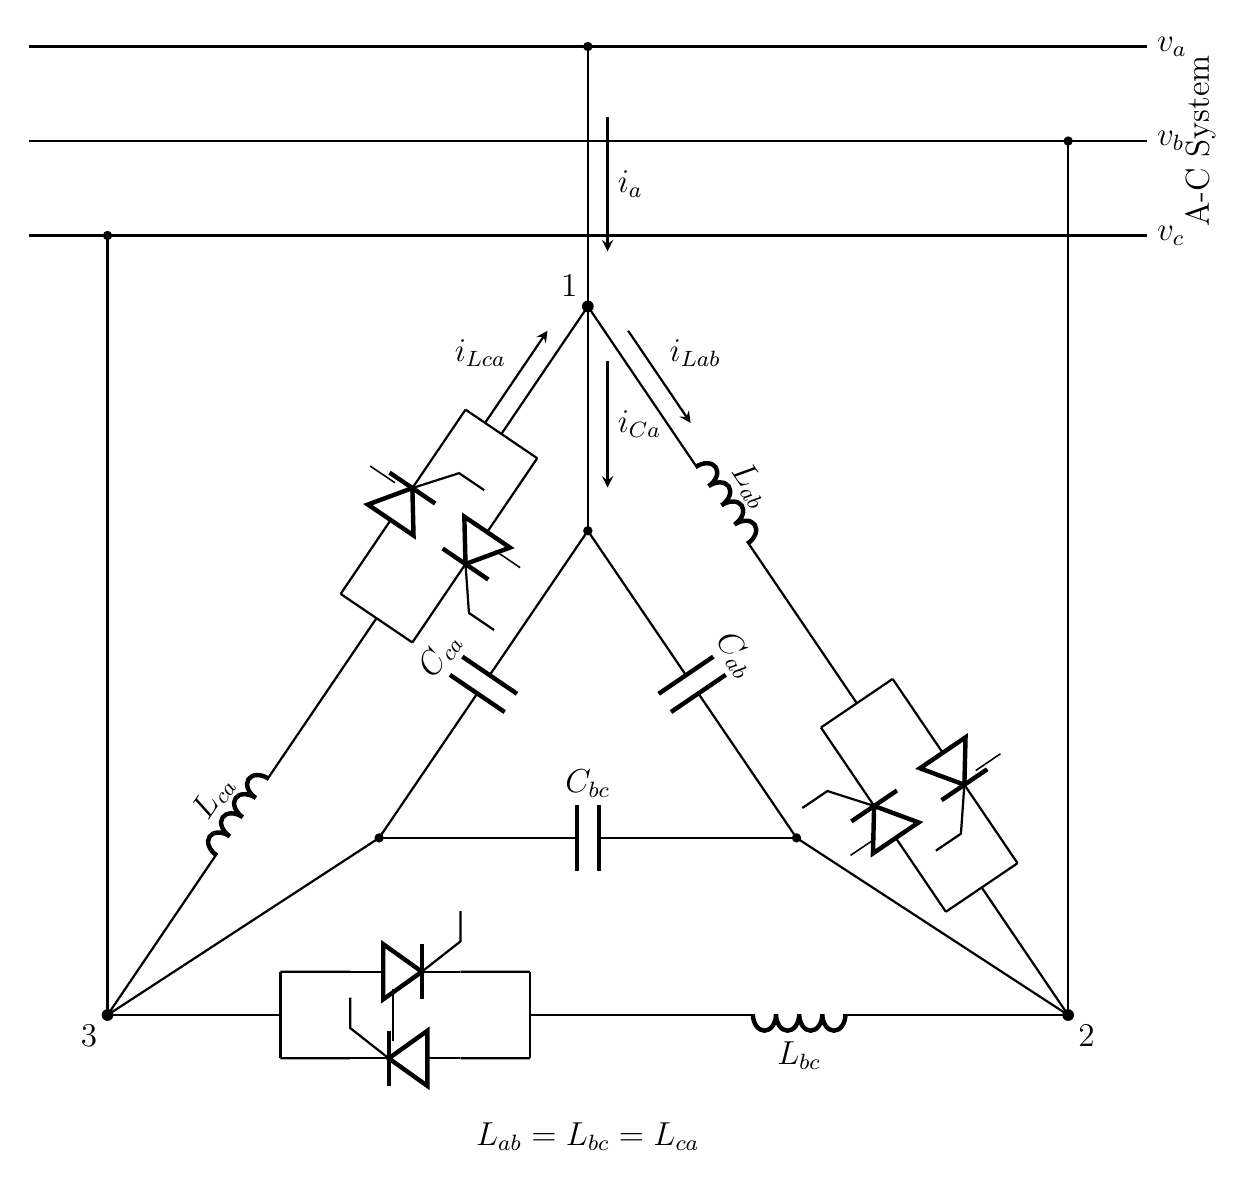
\begin{tikzpicture}[line width=0.8pt, every node/.style={font=\large}]

    % ==========================================
    % MACRO PARA O RAMO TCR (Indutor + Tiristores)
    % ==========================================
    % Desenha um indutor em série com um bloco de tiristores em antiparalelo.
    % #1: Nó inicial, #2: Nó final, #3: Label do indutor
    \newcommand{\drawTCR}[4]{
        % Coordenadas proporcionais ao longo do caminho
        \path (#1) -- (#2)
            coordinate[pos=0.20] (p1)
            coordinate[pos=0.36] (p2)
            coordinate[pos=0.56] (p3)
            coordinate[pos=0.82] (p4);

        % Fio inicial e indutor
        \draw (#1) -- (p1);
        \draw (p1) to[L, l=#3] (p2);
        \draw (p2) -- (p3);

        % Bloco de tiristores em antiparalelo, afastado do fio principal
        \coordinate (v_up) at ($(p3)!0.55cm!90:(p4)$);
        \coordinate (u_up) at ($(p4)!0.55cm!-90:(p3)$);
        \coordinate (v_dn) at ($(p3)!0.55cm!-90:(p4)$);
        \coordinate (u_dn) at ($(p4)!0.55cm!90:(p3)$);
        \coordinate (g_up) at ($(v_up)!0.55!(u_up)$);
        \coordinate (g_dn) at ($(v_dn)!0.55!(u_dn)$);

        \draw (p3) -- (v_up);
        \draw (p3) -- (v_dn);
        \draw (u_up) -- (p4);
        \draw (u_dn) -- (p4);
        \draw (v_up) to[Ty, mirror] (u_up);
        \draw (u_dn) to[Ty] (v_dn);

        % Gates destacados para fora do ramo, sem encostar no fio principal
        \draw[line width=0.55pt] ($(g_up)!0.22cm!#4:(u_up)$) -- ($(g_up)!0.60cm!#4:(u_up)$);
        \draw[line width=0.55pt] ($(g_dn)!0.22cm!#4:(v_dn)$) -- ($(g_dn)!0.60cm!#4:(v_dn)$);

        % Fio final
        \draw (p4) -- (#2);
    }

    % ==========================================
    % MACRO PARA SETAS DE CORRENTE PARALELAS
    % ==========================================
    \newcommand{\pararrow}[5]{
        \path (#1) -- (#2) coordinate[pos=#3] (as) coordinate[pos=#4] (ae);
        \coordinate (aso) at ($(as)!0.25cm!90:(#2)$);
        \coordinate (aeo) at ($(ae)!0.25cm!90:(#2)$);
        \draw[->, >=stealth] (aso) -- (aeo) node[midway, auto] {#5};
    }

    % ==========================================
    % COORDENADAS PRINCIPAIS DO SISTEMA
    % ==========================================
    % Vértices do Delta Externo
    \coordinate (N1) at (0, 3.3);
    \coordinate (N2) at (6.1, -5.7);
    \coordinate (N3) at (-6.1, -5.7);

    % Vértices do Delta Interno (Capacitores)
    \coordinate (J1) at (0, 0.45);
    \coordinate (J2) at (2.65, -3.45);
    \coordinate (J3) at (-2.65, -3.45);

    % ==========================================
    % SISTEMA A-C SUPERIOR E CONEXÕES
    % ==========================================
    \draw (-7.1, 6.6) -- (7.1, 6.6) node[right] {$v_a$};
    \draw (-7.1, 5.4) -- (7.1, 5.4) node[right] {$v_b$};
    \draw (-7.1, 4.2) -- (7.1, 4.2) node[right] {$v_c$};
    \node[rotate=90, anchor=south] at (8.1, 5.4) {A-C System};

    % Ligações dos nós principais às linhas A-C com nós (bolinhas)
    \draw (N1) -- (0, 6.6) node[circle,fill,inner sep=1.2pt, font=\normalsize]{};
    \draw (N2) -- (6.1, 5.4) node[circle,fill,inner sep=1.2pt, font=\normalsize]{};
    \draw (N3) -- (-6.1, 4.2) node[circle,fill,inner sep=1.2pt, font=\normalsize]{};

    % ==========================================
    % DELTA EXTERNO (TCR)
    % ==========================================
    % Desenhando os 3 ramos usando a macro criada
    \drawTCR{N1}{N2}{$L_{ab}$}{90}
    \drawTCR{N2}{N3}{$L_{bc}$}{-90}
    \drawTCR{N3}{N1}{$L_{ca}$}{90}

    % ==========================================
    % DELTA INTERNO (Fixed Capacitors)
    % ==========================================
    % Conexões dos vértices externos para os vértices internos
    \draw (N1) -- (J1);
    \draw (N2) -- (J2);
    \draw (N3) -- (J3);

    % Pontos (bolinhas) no delta interno
    \node[circle, fill=black, inner sep=1.2pt, font=\normalsize] at (J1) {};
    \node[circle, fill=black, inner sep=1.2pt, font=\normalsize] at (J2) {};
    \node[circle, fill=black, inner sep=1.2pt, font=\normalsize] at (J3) {};

    % Ramos dos Capacitores
    \draw (J1) to[C, l=$C_{ab}$] (J2);
    \draw (J2) to[C, l_=$C_{bc}$] (J3); % l_ inverte o lado do texto
    \draw (J3) to[C, l=$C_{ca}$] (J1);

    % ==========================================
    % RÓTULOS E CORRENTES
    % ==========================================
    % Numeração dos nós
    \node[circle, fill=black, inner sep=1.5pt, font=\normalsize] at (N1) {};
    \node[above left] at (N1) {1};
    
    \node[circle, fill=black, inner sep=1.5pt, font=\normalsize] at (N2) {};
    \node[below right] at (N2) {2};
    
    \node[circle, fill=black, inner sep=1.5pt, font=\normalsize] at (N3) {};
    \node[below left] at (N3) {3};

    % Setas de corrente manuais
    \draw[->, >=stealth] (0.25, 5.7) -- (0.25, 4.0) node[midway, right] {$i_a$};
    \draw[->, >=stealth] (0.25, 2.6) -- (0.25, 1.0) node[midway, right] {$i_{Ca}$};

    % Setas de corrente nos ramos do delta usando a macro paralela
    \pararrow{N1}{N2}{0.05}{0.18}{$i_{Lab}$}
    \pararrow{N3}{N1}{0.82}{0.95}{$i_{Lca}$}

    % ==========================================
    % EQUAÇÃO INFERIOR
    % ==========================================
    \node at (0, -7.25) {$L_{ab} = L_{bc} = L_{ca}$};

\end{tikzpicture}%
}
    \caption{SVC with each delta branch
    $\ell\in\{ab,bc,ca\}$ composed of capacitor bank $C_{j,\ell}$ in parallel
    with TCR controlled by the firing angle $\alpha_{j,\ell}$.}
    \label{fig:delta_fc_tcr_svc}
\end{figure}


At the fundamental frequency, the equivalent branch susceptance of an SVC connected at bus $j$ in
delta branch $\ell \in \{ab,bc,ca\}$ is expressed as

\begin{equation}
    B_{\mathrm{SVC},j,\ell}(\alpha_{j,\ell}) =
    B_{C,j,\ell} - B_{\mathrm{TCR},j,\ell}(\alpha_{j,\ell}),
    \label{eq:svc_susceptance}
\end{equation}

\noindent where $B_{C,j,\ell}$ denotes the fixed capacitor susceptance and
$B_{\mathrm{TCR},j,\ell}(\alpha_{j,\ell})$ represents the controllable
susceptance of the TCR. The latter depends on
the firing angle $\alpha_{j,\ell}$, which determines the conduction interval
of the thyristors. For a delta-connected SVC, each branch is subjected to the
corresponding line-to-line voltage. Thus, for a system with nominal
line-to-line voltage $V_{\mathrm{LL,nom}}$, the total reactive-power rating
of the compensator is calculated as

\begin{equation}
    Q_{\mathrm{SVC},j} = V_{\mathrm{LL,nom}}^2
    \sum_{\ell \in \{ab,bc,ca\}} \left|B_{\mathrm{SVC},j,\ell}\right|,
    \label{eq:svc_rating}
\end{equation}

\noindent where $V_{\mathrm{LL,nom}}$ is expressed in kV,
$B_{\mathrm{SVC},j,\ell}$ in siemens, and $Q_{\mathrm{SVC},j}$ in MVAr.


The harmonic current injection of the SVC is evaluated independently for
each delta branch. Then, the total current in branch $\ell$
at harmonic order $h$ is given by

\begin{equation}\small
    I_{\mathrm{SVC},j,\ell}^{(h)}
    =I_{\mathrm{C},j,\ell}^{(h)}+I_{\mathrm{TCR},j,\ell}^{(h)}
    =\mathrm{j}h\omega C_{j,\ell}V_{j,\ell}^{(h)}+
    I_{\mathrm{TCR},j,\ell}^{(h)}(v_{j,\ell},\alpha_{j,\ell}).
    \label{eq:svc_branch_current}
\end{equation}

 $I_{\mathrm{C},j,\ell}^{(h)}$ and
$I_{\mathrm{TCR},j,\ell}^{(h)}$ denote the capacitor and TCR current
phasors, respectively; $C_{j,\ell}$ is the branch capacitance;
$\omega=2\pi f$ is the fundamental angular frequency, with $f$ denoting
the system frequency; and $V_{j,\ell}^{(h)}$ is the voltage
phasor across branch $\ell$ at harmonic order $h$. The operator
$\mathrm{j}=\sqrt{-1}$ denotes the imaginary unit. Unlike the 
capacitor contribution, the TCR current depends nonlinearly on the
instantaneous branch voltage and on the firing angle.

To represent this nonlinear behavior, the TCR current waveform is
decomposed into its harmonic components through a Fourier series. For
branch $\ell$ of compensator $j$, the current is expressed as

\begin{equation}
    i_{j,\ell}(t)=
    \sum_{h\in\mathcal{H}}
    I_{j,\ell}^{(h)}(\alpha_{j,\ell})
    \cos\!\left(h\omega t+\phi_{j,\ell}^{(h)}\right),
    \label{eq:tcr_fourier}
\end{equation}

\noindent where $\mathcal{H}$ is the set of harmonic orders considered,
$I_{j,\ell}^{(h)}$ is the magnitude of the current component at harmonic
order $h$, and $\phi_{j,\ell}^{(h)}$ is its corresponding phase angle.
Both quantities depend on the firing angle and on the line-to-line voltage
applied to the TCR branch. The resulting branch currents are converted
into phase current injections through the delta incidence relation

\begin{equation}
    \begin{bmatrix}
        I_{j,a}^{(h)}\\ I_{j,b}^{(h)}\\ I_{j,c}^{(h)}
    \end{bmatrix}
    =
    \begin{bmatrix}
        1&0&-1\\ -1&1&0\\ 0&-1&1
    \end{bmatrix}
    \begin{bmatrix}
        I_{j,ab}^{(h)}\\ I_{j,bc}^{(h)}\\ I_{j,ca}^{(h)}
    \end{bmatrix},
    \label{eq:delta_incidence}
\end{equation}

\noindent where $I_{j,a}^{(h)}$, $I_{j,b}^{(h)}$, and
$I_{j,c}^{(h)}$ are the harmonic current injections into phases $a$,
$b$, and $c$, respectively, whereas $I_{j,ab}^{(h)}$,
$I_{j,bc}^{(h)}$, and $I_{j,ca}^{(h)}$ represent the corresponding
delta-branch current phasors. This relationship shows that each phase
current injection is obtained from the difference between the currents
of its two adjacent delta branches.

For a balanced SVC, the three branches have identical electrical
parameters and firing angles, such that
$\alpha_{j,ab}=\alpha_{j,bc}=\alpha_{j,ca}=\alpha_j$.
Under balanced line-to-line voltages, the branch harmonic phasors have
equal magnitudes and phase displacements determined by the harmonic
order. Consequently, triplen harmonic currents cancel at the delta
terminals and are ideally confined within the delta connection.

Conversely, when independent firing angles are employed, the branch
currents are no longer characterized by a single harmonic magnitude
and a set of fixed phase displacements. Instead, their harmonic
phasors must be evaluated individually as

\begin{equation}
    \begin{bmatrix}
        I_{j,ab}^{(h)}\\
        I_{j,bc}^{(h)}\\
        I_{j,ca}^{(h)}
    \end{bmatrix}
    =
    \begin{bmatrix}
        I_{j,ab}^{(h)}(\alpha_{j,ab})\\
        I_{j,bc}^{(h)}(\alpha_{j,bc})\\
        I_{j,ca}^{(h)}(\alpha_{j,ca})
    \end{bmatrix}.
    \label{eq:unbalanced_branch_phasors}
\end{equation}

This independent control allows the SVC to introduce fundamental-frequency
asymmetries that can compensate for the negative-sequence voltage caused
by unbalanced loads. However, unequal firing angles also modify the
magnitudes and phase angles of the branch harmonic currents, potentially
introducing additional positive- and negative-sequence harmonic
components into the feeder. Therefore, phase balancing and harmonic
performance cannot be treated as independent objectives. In the proposed
optimization framework, the firing angles are selected while explicitly
constraining the voltage total harmonic distortion, $\mathrm{THD}_V$,
to ensure that the harmonic distortion resulting from the independent
branch control remains within the prescribed limits.



The harmonic current injections are calculated from the Fourier
coefficients of the TCR current over its respective conduction intervals.
To obtain these coefficients, the instantaneous line-to-line voltage
applied to each branch is first reconstructed from its harmonic components.
For branch $\ell$ of compensator $j$, this voltage is expressed as

\begin{equation}
    v_{j,\ell}(t)=
    \sum_{n\in\mathcal{H}}
    \left[V_{r,j,\ell}^{(n)}\cos(n\omega t)+
    V_{m,j,\ell}^{(n)}\sin(n\omega t)\right].
    \label{eq:branch_voltage_waveform}
\end{equation}

Here, $V_{r,j,\ell}^{(n)}$ and $V_{m,j,\ell}^{(n)}$ are the real and
imaginary rectangular components of the branch voltage phasor at harmonic
order $n$, respectively. The summation reconstructs the instantaneous
voltage waveform from all harmonic orders included in $\mathcal{H}$.

The reconstructed voltage is used to determine the TCR current during
each thyristor conduction interval
$[t_{0,j,\ell}^{s},t_{f,j,\ell}^{s}]$, where
$s\in\{1,2\}$ identifies the two firing intervals within each fundamental
period. The firing angle $\alpha_{j,\ell}$ determines the thyristor
turn-on instant $t_{0,j,\ell}^{s}$, whereas
$t_{f,j,\ell}^{s}$ denotes the corresponding current extinction instant.

Let $\theta_\ell$ denote the angular reference associated with the
line-to-line voltage of delta branch $\ell$. For the adopted phase
convention, the reference angles are
$\theta_{ab}=\pi/6$, $\theta_{bc}=-\pi/2$, and
$\theta_{ca}=5\pi/6$. Accordingly, the firing instants during the
$q$th fundamental period are given by

\begin{subequations}
\label{eq:firing_instants}
\begin{align}
    t_{0,j,\ell}^{1}(q)&=
    \frac{2\pi q+\theta_{\ell}+\alpha_{j,\ell}}{\omega},\\
    t_{0,j,\ell}^{2}(q)&=
    \frac{2\pi q+\theta_{\ell}+\pi+\alpha_{j,\ell}}{\omega}.
\end{align}
\end{subequations}

Thus, increasing $\alpha_{j,\ell}$ delays the thyristor turn-on instant
with respect to the corresponding branch-voltage reference. Under the
symmetric ideal TCR approximation, the current extinction instants are
assumed to occur at the firing-symmetric boundaries

\begin{subequations}
\label{eq:extinction_instants}
\begin{align}
    t_{f,j,\ell}^{1}(q)&=
    \frac{2\pi q+\theta_{\ell}+2\pi-\alpha_{j,\ell}}{\omega},\\
    t_{f,j,\ell}^{2}(q)&=
    \frac{2\pi q+\theta_{\ell}+3\pi-\alpha_{j,\ell}}{\omega}.
\end{align}
\end{subequations}

Fig.~\ref{figrtc} illustrates the TCR conduction behavior as a function
of the thyristor firing angle.

\begin{figure}[htpb!]
    \centering
    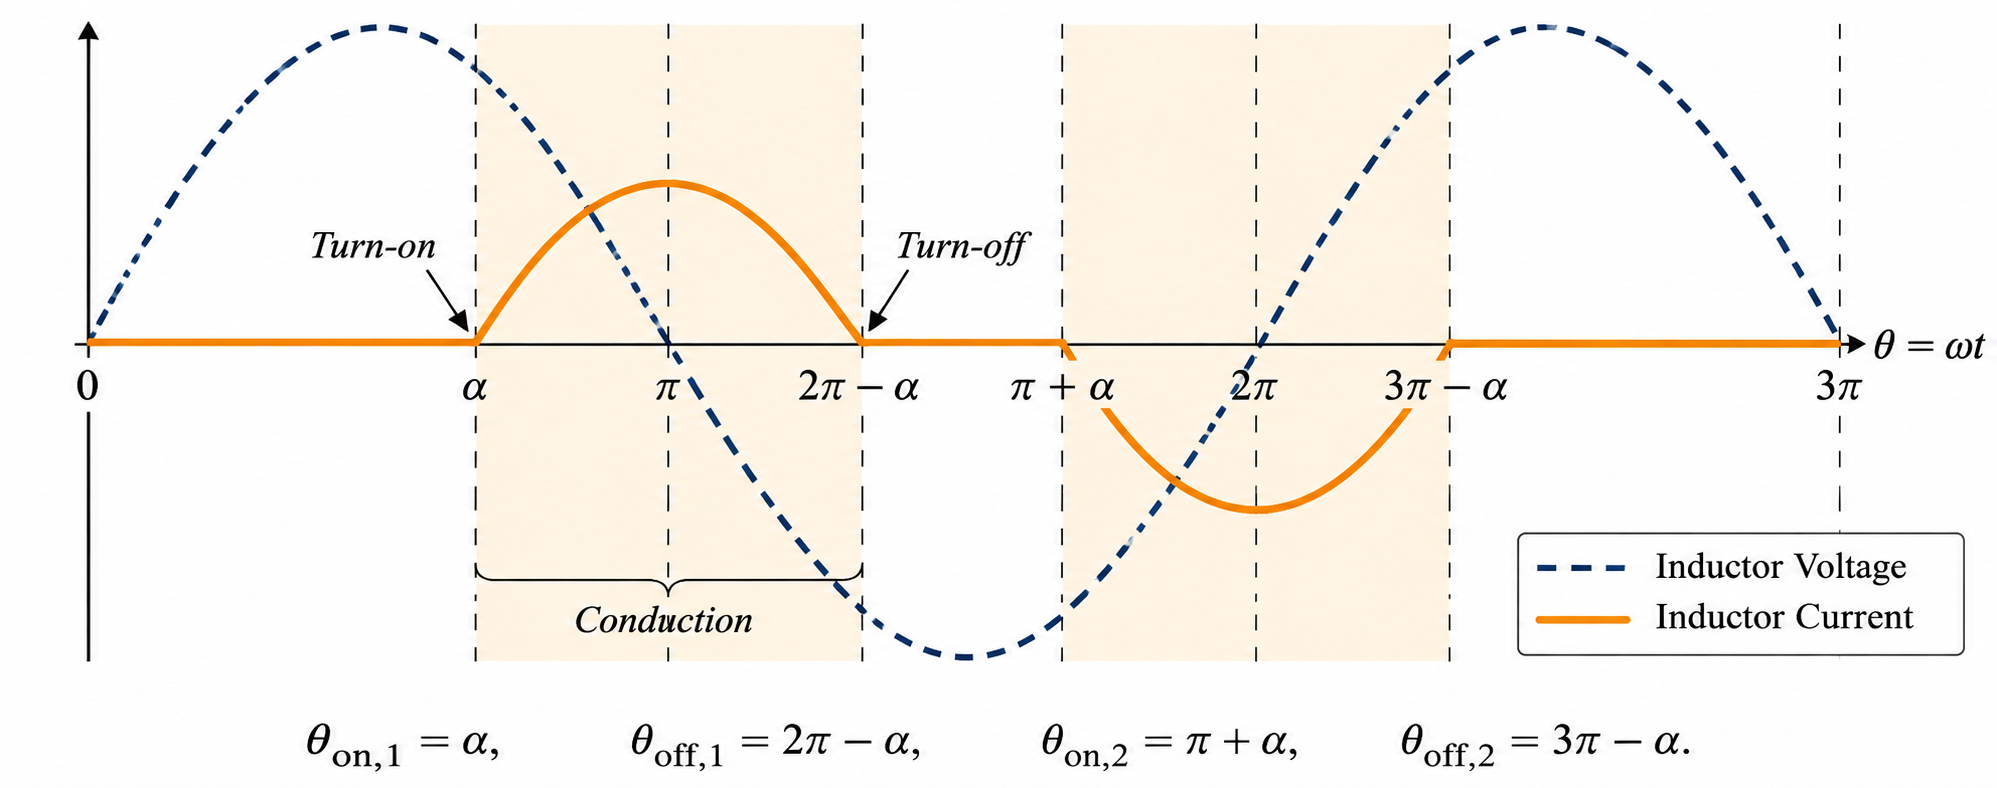
\includegraphics[width=1.05\linewidth]{0b282cfd-d955-475b-9c7b-df4687952566.png}
    \caption{TCR conduction intervals as a function of the thyristor
    firing angle.}
    \label{figrtc}
\end{figure}

The firing and extinction instants define the conduction intervals
of the TCR. The corresponding conduction angle is
$\sigma_{j,\ell}=2(\pi-\alpha_{j,\ell})$, which varies from zero
at $\alpha_{j,\ell}=\pi$ to its maximum value of $\pi$ at
$\alpha_{j,\ell}=\pi/2$. Within each conduction interval, the
reactor current is governed by the differential equation

\begin{equation}
    L_{j,\ell}\frac{\mathrm{d}i_{j,\ell}^{s}(t)}{\mathrm{d}t}
    +R_{j,\ell}i_{j,\ell}^{s}(t)=v_{j,\ell}(t),
    \qquad t_{0,j,\ell}^{s}\leq t\leq t_{f,j,\ell}^{s}.
    \label{eq:tcr_differential}
\end{equation}

In~\eqref{eq:tcr_differential}, $L_{j,\ell}$ and $R_{j,\ell}$ are the
inductance and resistance of the TCR reactor, respectively;
$i_{j,\ell}^{s}(t)$ is its instantaneous current during conduction
interval $s$; and $v_{j,\ell}(t)$ is the applied line-to-line voltage
defined in~\eqref{eq:branch_voltage_waveform}.

By substituting the harmonic voltage representation into the
differential equation, the analytical current response can be written as

\begin{equation}
\begin{aligned}
    i_{j,\ell}^{s}(t)=&K_{j,\ell}^{s}
    e^{-R_{j,\ell}(t-t_{0,j,\ell}^{s})/L_{j,\ell}}\\
    &+\sum_{n\in\mathcal{H}}
    \frac{V_{r,j,\ell}^{(n)}}{Z_{n,j,\ell}}
    \cos(n\omega t-\varphi_{n,j,\ell})\\
    &+\sum_{n\in\mathcal{H}}
    \frac{V_{m,j,\ell}^{(n)}}{Z_{n,j,\ell}}
    \sin(n\omega t-\varphi_{n,j,\ell}),
\end{aligned}
\label{eq:tcr_analytical_current}
\end{equation}

\noindent where $Z_{n,j,\ell}=
    \sqrt{R_{j,\ell}^{2}+(n\omega L_{j,\ell})^{2}},$ and $\varphi_{n,j,\ell}=
    \tan^{-1}\left(\frac{n\omega L_{j,\ell}}{R_{j,\ell}}\right).$ Here, $Z_{n,j,\ell}$ is the magnitude of the reactor impedance at
harmonic order $n$, and $\varphi_{n,j,\ell}$ is its corresponding
impedance phase angle. The summation terms describe the forced response
of the R--L branch to the individual harmonic voltage components,
whereas the exponential term represents the natural response associated
with the initial condition at the thyristor turn-on instant.
The integration constant $K_{j,\ell}^{s}$ is determined from the
initial condition of the reactor current.

Since the thyristor blocks the reactor before firing, the current at the
beginning of each conduction interval is assumed to be zero, i.e.,
$i_{j,\ell}^{s}(t_{0,j,\ell}^{s})=0$. Applying this condition to
\eqref{eq:tcr_analytical_current} yields

\begin{equation}
\begin{aligned}
    K_{j,\ell}^{s}=&-
    \sum_{n\in\mathcal{H}}
    \frac{V_{r,j,\ell}^{(n)}}{Z_{n,j,\ell}}
    \cos(n\omega t_{0,j,\ell}^{s}-\varphi_{n,j,\ell})\\
    &-
    \sum_{n\in\mathcal{H}}
    \frac{V_{m,j,\ell}^{(n)}}{Z_{n,j,\ell}}
    \sin(n\omega t_{0,j,\ell}^{s}-\varphi_{n,j,\ell}).
\end{aligned}
\label{eq:tcr_initial_constant}
\end{equation}

With the integration constant determined, the real and imaginary
Fourier coefficients of the TCR current at harmonic order $h>0$
can be calculated by integrating the instantaneous current over
the two conduction intervals. Following the adopted phasor convention,
these coefficients are defined as

\begin{subequations}
\label{eq:tcr_fourier_coefficients}
\begin{align}
    I_{r,\mathrm{TCR},j,\ell}^{(h)}
    &=\frac{\omega}{\pi}\sum_{s=1}^{2}
    \int_{t_{0,j,\ell}^{s}}^{t_{f,j,\ell}^{s}}
    i_{j,\ell}^{s}(t)\cos(h\omega t)\,\mathrm{d}t,\\
    I_{m,\mathrm{TCR},j,\ell}^{(h)}
    &=-\frac{\omega}{\pi}\sum_{s=1}^{2}
    \int_{t_{0,j,\ell}^{s}}^{t_{f,j,\ell}^{s}}
    i_{j,\ell}^{s}(t)\sin(h\omega t)\,\mathrm{d}t.
\end{align}
\end{subequations}

The factor $\omega/\pi$ accounts for the Fourier normalization over
one fundamental period, while the negative sign in the imaginary
coefficient ensures consistency with the adopted rectangular phasor
convention. Specifically,
$I_{\mathrm{TCR},j,\ell}^{(h)}
=I_{r,\mathrm{TCR},j,\ell}^{(h)}
+\mathrm{j}I_{m,\mathrm{TCR},j,\ell}^{(h)}$.

Substituting the analytical current expression in
\eqref{eq:tcr_analytical_current} into
\eqref{eq:tcr_fourier_coefficients} allows the integrals to be
evaluated in closed form. To simplify the notation, the branch indices
$(j,\ell)$ are temporarily omitted from the auxiliary expressions.
Define

\begin{subequations}
\label{eq:tcr_forced_coefficients}
\begin{align}
    A_n&=\frac{V_{r,j,\ell}^{(n)}\cos\varphi_{n,j,\ell}
    -V_{m,j,\ell}^{(n)}\sin\varphi_{n,j,\ell}}{Z_{n,j,\ell}},\\
    B_n&=\frac{V_{r,j,\ell}^{(n)}\sin\varphi_{n,j,\ell}
    +V_{m,j,\ell}^{(n)}\cos\varphi_{n,j,\ell}}{Z_{n,j,\ell}}.
\end{align}
\end{subequations}

Here, $A_n$ and $B_n$ are the cosine and sine coefficients,
respectively, of the forced current response at harmonic order $n$.
Consequently, the forced component of the reactor current becomes

\[
    \sum_{n\in\mathcal H}
    \left[A_n\cos(n\omega t)+B_n\sin(n\omega t)\right].
\]

Note that $B_n$ denotes a Fourier sine coefficient and is unrelated
to the susceptance notation used in the SVC model.

For any integer $k$, the following endpoint functions are introduced
to represent the integrals of the trigonometric terms over each
conduction interval:

\begin{subequations}
\label{eq:tcr_endpoint_kernels}
\begin{align}
    \mathcal C_k^s&=
    \begin{cases}
    \displaystyle\frac{\sin(k\omega t_f^s)-\sin(k\omega t_0^s)}
    {k\omega},&k\ne0,\\[2mm]
    t_f^s-t_0^s,&k=0,
    \end{cases}\\
    \mathcal S_k^s&=
    \begin{cases}
    \displaystyle\frac{\cos(k\omega t_0^s)-\cos(k\omega t_f^s)}
    {k\omega},&k\ne0,\\[2mm]
    0,&k=0.
    \end{cases}
\end{align}
\end{subequations}

In these expressions, $t_0^s$ and $t_f^s$ denote the initial and
final instants of conduction interval $s$, respectively. The functions
$\mathcal C_k^s$ and $\mathcal S_k^s$ correspond to the definite
integrals of $\cos(k\omega t)$ and $\sin(k\omega t)$ over that interval.
Their definitions for $k=0$ avoid division by zero when the difference
between two harmonic orders vanishes.

The natural response, represented by the exponential term in
\eqref{eq:tcr_analytical_current}, is handled through the auxiliary
functions

\begin{subequations}
\label{eq:tcr_exponential_kernels}
\begin{align}
    \mathcal E_{c,h}^s
    &=\left[
    \frac{e^{-a(t-t_0^s)}
    \bigl[-a\cos(h\omega t)+h\omega\sin(h\omega t)\bigr]}
    {a^2+(h\omega)^2}
    \right]_{t_0^s}^{t_f^s},\\
    \mathcal E_{s,h}^s
    &=\left[
    \frac{e^{-a(t-t_0^s)}
    \bigl[-a\sin(h\omega t)-h\omega\cos(h\omega t)\bigr]}
    {a^2+(h\omega)^2}
    \right]_{t_0^s}^{t_f^s},
\end{align}
\end{subequations}

where $a=R_{j,\ell}/L_{j,\ell}$ is the exponential decay coefficient,
and the notation
$[F(t)]_{t_0^s}^{t_f^s}=F(t_f^s)-F(t_0^s)$ denotes evaluation
at the interval endpoints. The functions $\mathcal E_{c,h}^s$
and $\mathcal E_{s,h}^s$ provide the analytical integrals of the
exponential natural response multiplied by the cosine and sine
Fourier basis functions, respectively.

By applying the trigonometric product-to-sum identities, the Fourier
coefficients can be expressed entirely in terms of the previously
defined endpoint functions. With $K^s=K_{j,\ell}^s$, the resulting
closed-form expressions are

\begin{subequations}\small
\label{eq:tcr_fourier_closed_form}
\begin{align}
    I_{r,\mathrm{TCR},j,\ell}^{(h)}
    &=\frac{\omega}{\pi}\sum_{s=1}^{2}
    \Biggl\{K^s\mathcal E_{c,h}^s\nonumber\\
    &\quad+\frac{1}{2}\sum_{n\in\mathcal H}
    \Bigl[A_n\bigl(\mathcal C_{n-h}^s+\mathcal C_{n+h}^s\bigr)
    +B_n\bigl(\mathcal S_{n+h}^s+\mathcal S_{n-h}^s\bigr)\Bigr]\Biggr\},\\
    I_{m,\mathrm{TCR},j,\ell}^{(h)}
    &=-\frac{\omega}{\pi}\sum_{s=1}^{2}
    \Biggl\{K^s\mathcal E_{s,h}^s\nonumber\\
    &\quad+\frac{1}{2}\sum_{n\in\mathcal H}
    \Bigl[A_n\bigl(\mathcal S_{n+h}^s-\mathcal S_{n-h}^s\bigr)
    +B_n\bigl(\mathcal C_{n-h}^s-\mathcal C_{n+h}^s\bigr)\Bigr]\Biggr\}.
\end{align}
\end{subequations}

Equations~\eqref{eq:tcr_fourier_closed_form} provide an analytical
evaluation of the TCR harmonic current coefficients using only finite
summations and endpoint evaluations, thus avoiding numerical
integration over the conduction intervals. In particular, when
$n=h$, the definitions $\mathcal C_0^s=t_f^s-t_0^s$ and
$\mathcal S_0^s=0$ must be used to avoid singular expressions involving
$(n-h)\omega$ in the denominator. Moreover, for $h>0$, the exponential
kernels remain well defined when $R_{j,\ell}=0$, since their
denominator reduces to $(h\omega)^2$.

These expressions evaluate the current over the prescribed conduction
intervals defined by the firing and extinction instants. If the
extinction instants are instead determined from the actual zero
crossings of the reactor current, the same analytical expressions
remain applicable, provided that the corresponding extinction
instants are used as integration limits. For positive harmonic orders, the complex TCR current phasor is
assembled as $I_{\mathrm{TCR},j,\ell}^{(h)}
    =
    I_{r,\mathrm{TCR},j,\ell}^{(h)}
    +\mathrm{j}I_{m,\mathrm{TCR},j,\ell}^{(h)}.$

 The capacitor contribution in
\eqref{eq:svc_branch_current} is represented through the corresponding
admittance stamp in the admittance matrix representing the power system to be analyzed, whereas the TCR harmonic
coefficients obtained from \eqref{eq:tcr_fourier_coefficients}
constitute the nonlinear SVC current-injection term
$\bm{g}_{\mathrm{SVC}}$. The resulting branch currents are converted
into phase current injections through the delta incidence matrix
in~\eqref{eq:delta_incidence}. This formulation preserves the
independent control of the three firing angles
$\alpha_{j,ab}$, $\alpha_{j,bc}$, and $\alpha_{j,ca}$ while
consistently accounting for their effects on both the fundamental
and harmonic components of the feeder currents.



\subsection{The Proposed Optimization Model}

For a given operating point, defined by the network topology, electrical
parameters, and load data, an optimal control problem is formulated to
determine the settings of the controllable SVC devices.

Let $\mathcal{S}_c$ denote the set of controllable SVC devices,
$\Phi=\{a,b,c\}$ the set of phase indices, and
$\mathcal{L}=\{ab,bc,ca\}$ the set of delta branches. The decision
vector is therefore defined as

\begin{equation}
    \bm{\alpha}=
    \left[\alpha_{j,\ell}\right]_{j\in\mathcal{S}_c,\,\ell\in\mathcal{L}}^{\top}
    \in\mathbb{R}^{|\mathcal{S}_c||\mathcal{L}|}.
    \label{eq:decision_vector}
\end{equation}

Each component $\alpha_{j,\ell}$ represents the firing angle of branch
$\ell$ of SVC $j$. The fundamental-frequency voltage
phasors and the harmonic voltage components are the electrical state
variables determined by the HTPCIM equations for a given control vector.
Thus, the voltage solution is implicitly dependent on the selected
firing angles, i.e., $\bm{V}=\bm{V}(\bm{\alpha})$.

The optimization aims to minimize a voltage-regulation objective while
satisfying the electrical operating constraints of the distribution
system. These constraints include fundamental-frequency voltage limits,
maximum voltage total harmonic distortion, voltage-unbalance limits,
firing-angle bounds, and the current-balance equations associated with
the fundamental and harmonic power-flow solutions. The resulting
optimization problem is expressed as

\begin{subequations}
\label{eq:optimization_problem}
\begin{align}
    \underset{\bm{\alpha},\bm{V}}{\operatorname{minimize}}\quad
    &J(\bm{\alpha},\bm{V})\\
    \text{subject to}\quad
    &V^{\min}\leq |V_{i,\phi}^{(1)}|\leq V^{\max},
    &&\forall i\in\mathcal{B}_c,\ \forall\phi\in\Phi,\\
    &\mathrm{THD}_{V,i,\phi}\leq\mathrm{THD}_{V}^{\max},
    &&\forall i\in\mathcal{B},\ \forall\phi\in\Phi,\\
    &\mathrm{VUF}_{i}\leq\mathrm{VUF}^{\max},
    &&\forall i\in\mathcal{B}_c,\\
    &\alpha^{\min}\leq\alpha_{j,\ell}\leq\alpha^{\max},
    &&\forall j\in\mathcal{S}_c,\ \forall\ell\in\mathcal{L},\\
    &\Delta I_{r,i,\phi}^{(h)}=0,
    &&\forall i\in\mathcal{B},\ \forall\phi\in\Phi,\ \forall h\in\mathcal{H},\\
    &\Delta I_{m,i,\phi}^{(h)}=0,
    &&\forall i\in\mathcal{B},\ \forall\phi\in\Phi,\ \forall h\in\mathcal{H}.
\end{align}
\end{subequations}

In the formulation, $\mathcal{B}=\{1,\ldots,N_b\}$ denotes the set of system buses,
where $N_b$ is the total number of buses, and
$\mathcal{B}_c\subseteq\mathcal{B}$ identifies the buses whose voltages
are regulated by the controller. The quantities $V^{\min}$ and
$V^{\max}$ are the lower and upper admissible fundamental-frequency
voltage magnitudes, respectively, expressed in per unit. The parameter
$\mathrm{THD}_{V}^{\max}$ specifies the maximum admissible voltage total
harmonic distortion, whereas $\mathrm{VUF}^{\max}$ defines the maximum
voltage-unbalance factor. Finally, $\alpha^{\min}$ and
$\alpha^{\max}$ establish the admissible firing-angle interval for
each TCR branch. The HTPCIM  load flow current-mismatch equalities enforce the
electrical consistency of the solution at every harmonic order
considered in the analysis.

\subsubsection{Reduced-Space Formulation}
\label{subsec:reduced_space}

The variables of the optimization problem can be partitioned into control
and state variables. The firing-angle vector $\bm{\alpha}$ contains the
independent control variables because its components are settings that can
be directly assigned to the SVC branches within their admissible bounds. In
contrast, the fundamental and harmonic bus voltages are state variables.
They cannot be independently selected by the optimizer because, once
$\bm{\alpha}$, the loads, and the network parameters are fixed, their values
must satisfy Kirchhoff's laws and the nonlinear current-injection equations
at all harmonic orders. Hence, the state variables describe the electrical
response of the network to a chosen control action, whereas the control
variables describe the action itself.

The formulation in~\eqref{eq:optimization_problem} is a full-space
representation because it displays both the SVC controls and the harmonic
voltages as optimization variables, while the HTPCIM current-balance
equations appear explicitly as equality constraints. In a multifrequency
network model, this representation introduces thousands of electrical-state
variables and the same number of balance equations, even though the number
of SVC controls is comparatively small. Carrying all these variables into
each SQP subproblem would substantially increase its dimension and would
require the optimizer to recover feasibility of the network equations along
with the operational constraints.

The reduced-space formulation is adopted to avoid this unnecessary
optimization burden. Since the harmonic voltage state is determined by the
HTPCIM solution for a given firing-angle vector, the electrical states can be
eliminated as independent optimization variables. The SQP algorithm then
operates only on the firing angles, producing smaller quadratic subproblems,
while each state evaluation remains consistent with the nonlinear
multifrequency current-balance equations. This formulation also permits the
reuse of the HTPCIM Jacobian when computing control sensitivities and reduces
the need for repeated nonlinear power-flow solutions. These are the main
computational motivations for using reduced space in the proposed method,
following the classical reduced-gradient concept introduced for optimal
power flow and its more recent feasible reduced-space developments
\cite{DommelTinney1968,Pacaud2022ReducedSpace}.

To formalize this reduction, let
$\bm{y}$ collect the real and imaginary parts of all active bus-phase
voltages at every harmonic order considered, and write the simultaneous
multifrequency current mismatches as
\begin{equation}
    \bm{F}(\bm{y},\bm{\alpha})=\bm{0}.
    \label{eq:htpcim_state_equations}
\end{equation}
Consider a converged operating point
$(\overline{\bm{y}},\overline{\bm{\alpha}})$ such that
$\bm{F}(\overline{\bm{y}},\overline{\bm{\alpha}})=\bm{0}$. For a fixed and
smooth TCR operating regime, assume that $\bm{F}$ is continuously
differentiable in a neighborhood of this point and that the square state
Jacobian
$\bm{F}_{\bm{y}}=\partial\bm{F}/\partial\bm{y}$ is nonsingular at
$(\overline{\bm{y}},\overline{\bm{\alpha}})$. The implicit-function theorem
then guarantees the existence of neighborhoods around
$\overline{\bm{\alpha}}$ and $\overline{\bm{y}}$, together with a unique
continuously differentiable local mapping
$\bm{y}=\bm{y}(\bm{\alpha})$, such that
\begin{equation}
    \bm{y}(\overline{\bm{\alpha}})=\overline{\bm{y}},
    \qquad
    \bm{F}\bigl(\bm{y}(\bm{\alpha}),\bm{\alpha}\bigr)=\bm{0}.
    \label{eq:implicit_state_map}
\end{equation}
In the proposed application, this mapping does not need to be available in
closed form. For every trial value of $\bm{\alpha}$, Newton's method computes
$\bm{y}(\bm{\alpha})$ by solving the nonlinear HTPCIM equations for all
harmonic orders simultaneously. The theorem provides the local mathematical
justification for treating this numerical state solution as a differentiable
function of the SVC controls.

Under this regularity condition, replacing $\bm{y}$ by
$\bm{y}(\bm{\alpha})$ does not remove any physical equation or introduce an
approximation into the network model. Locally, every feasible full-space
pair $(\bm{y},\bm{\alpha})$ satisfying
$\bm{F}(\bm{y},\bm{\alpha})=\bm{0}$ corresponds to a point in the reduced
control space, and every reduced-space control vector for which the HTPCIM
converges generates the corresponding feasible full-space pair. The
objective and operational constraints are merely evaluated after this
implicit substitution. Therefore, the fundamental and harmonic couplings,
the nonlinear load equations, and the SVC current injections remain exactly
the same as in the full-space formulation; only the numerical coordinates
used by the optimizer are changed. The equivalence is local and assumes a
well-defined state solution. Near singular state Jacobians, multiple power-
flow solutions, or nonsmooth changes in the TCR operating condition, the
selected solution branch and the validity of the local sensitivities must be
examined explicitly.

Let $\widehat{J}(\bm{y},\bm{\alpha})$ denote the objective function and let
$\widehat{\bm{g}}(\bm{y},\bm{\alpha})$ collect the voltage-magnitude, THD,
VUF, and other operating inequalities. After eliminating the electrical
state through~\eqref{eq:htpcim_state_equations}, the reduced problem becomes
\begin{equation}
\begin{aligned}
    \underset{\bm{\alpha}}{\operatorname{minimize}}\quad
    &J_r(\bm{\alpha})
      =\widehat{J}\bigl(\bm{y}(\bm{\alpha}),\bm{\alpha}\bigr)\\
    \text{subject to}\quad
    &\bm{g}_r(\bm{\alpha})
      =\widehat{\bm{g}}\bigl(\bm{y}(\bm{\alpha}),\bm{\alpha}\bigr)
      \leq\bm{0},\\
    &\bm{\alpha}^{\min}\leq\bm{\alpha}\leq\bm{\alpha}^{\max}.
\end{aligned}
\label{eq:reduced_optimization_problem}
\end{equation}
Thus, the current-balance equations are not discarded: they are satisfied
internally whenever the state $\bm{y}(\bm{\alpha})$ is evaluated.

The dependence of the harmonic state on the firing angles is obtained by
differentiating~\eqref{eq:htpcim_state_equations}:
\begin{equation}
    \bm{F}_{\bm{y}}
    \frac{\mathrm{d}\bm{y}}{\mathrm{d}\bm{\alpha}}
    +\bm{F}_{\bm{\alpha}}=\bm{0},
    \qquad
    \frac{\mathrm{d}\bm{y}}{\mathrm{d}\bm{\alpha}}
    =-\bm{F}_{\bm{y}}^{-1}\bm{F}_{\bm{\alpha}},
    \quad
    \bm{F}_{\bm{\alpha}}
    =\frac{\partial\bm{F}}{\partial\bm{\alpha}}.
    \label{eq:reduced_state_sensitivity}
\end{equation}
The reduced first derivatives used by the optimizer then follow from the
chain rule:
\begin{align}
    \nabla_{\bm{\alpha}}J_r
    &=\widehat{J}_{\bm{\alpha}}
      +\widehat{J}_{\bm{y}}
       \frac{\mathrm{d}\bm{y}}{\mathrm{d}\bm{\alpha}},
       \label{eq:reduced_objective_gradient}\\
    \frac{\mathrm{d}\bm{g}_r}{\mathrm{d}\bm{\alpha}}
    &=\widehat{\bm{g}}_{\bm{\alpha}}
      +\widehat{\bm{g}}_{\bm{y}}
       \frac{\mathrm{d}\bm{y}}{\mathrm{d}\bm{\alpha}}.
       \label{eq:reduced_constraint_gradient}
\end{align}
In practice, the inverse in~\eqref{eq:reduced_state_sensitivity} is not
formed explicitly. Instead, the already assembled state Jacobian is
factorized and linear systems with the columns of
$-\bm{F}_{\bm{\alpha}}$ as right-hand sides are solved.

Compared with estimating each derivative through black-box perturbations,
the multiple-right-hand-side calculation in
\eqref{eq:reduced_state_sensitivity} avoids recomputing a complete nonlinear
HTPCIM solution for every individual firing-angle perturbation. This benefit
is especially relevant because the harmonic state may contain thousands of
real variables, whereas there are only three controls per SVC. The resulting
sensitivities are local; therefore, when a firing-angle change crosses a
nonsmooth TCR operating boundary, the state and its derivatives must be
reevaluated at the new operating point.

\subsubsection{Load Modeling and Current Injections}

The voltage-dependent load components are represented by the ZIP
model. The active-power injection is expressed as
\begin{equation}
P_{\chi,i,\phi}
=P_{i,\phi}^{nom}\left[
p_p+p_i\frac{|V_{i,\phi}^{(1)}|}{V_{i,\phi}^{nom}}
+p_z\left(\frac{|V_{i,\phi}^{(1)}|}{V_{i,\phi}^{nom}}\right)^2
\right],
\label{eq:zip_model}
\end{equation}
where $P_{i,\phi}^{nom}$ is the signed nominal active-power injection,
$V_{i,\phi}^{nom}$ is the nominal phase-to-neutral voltage magnitude,
and $p_p$, $p_i$, and $p_z$ are the constant-power,
constant-current, and constant-impedance fractions, respectively,
satisfying $p_p+p_i+p_z=1$. The reactive-power injection is defined
analogously.

The corresponding complex powers are converted into current
injections. The rectangular components of this current are consequently given by

\begin{subequations}
\label{eq:load_current_rectangular}
\begin{align}
    I_{\chi,r,i,\phi}^{(1)}&=
    \frac{P_{\chi,i,\phi}V_{r,i,\phi}^{(1)}+
    Q_{\chi,i,\phi}V_{m,i,\phi}^{(1)}}
    {\left(V_{i,\phi}^{(1)}\right)^2},\\
    I_{\chi,m,i,\phi}^{(1)}&=
    \frac{P_{\chi,i,\phi}V_{m,i,\phi}^{(1)}-
    Q_{\chi,i,\phi}V_{r,i,\phi}^{(1)}}
    {\left(V_{i,\phi}^{(1)}\right)^2},
\end{align}
\end{subequations}

\noindent where $V_{r,i,\phi}^{(1)}$ and $V_{m,i,\phi}^{(1)}$ are the real and
imaginary components of the fundamental voltage phasor, respectively,
and the subscripts $r$ and $m$ identify the real and imaginary
components of the corresponding current injection.





At the fundamental frequency, the aggregate nonlinear and prescribed
current injection at bus $i$ and phase $\phi$ is defined as

\begin{equation}
    I_{\mathrm{dev},i,\phi}^{(1)}=
    I_{\mathrm{\chi},i,\phi}^{(1)}+
    I_{\mathrm{TCR},i,\phi}^{(1)}
    \label{eq:aggregate_fundamental_current}
\end{equation}


$I_{\mathrm{dev},i,\phi}^{(1)}$ is the net complex
fundamental-frequency current injection at bus $i$ and phase $\phi$.
The terms on the right-hand side represent, respectively, the
 load current and the
TCR current.



The HTPCIM equations are incorporated into the optimization as
equality constraints. At the fundamental frequency, the real and
imaginary current mismatches are defined as

\begin{subequations}\small
\label{eq:fundamental_mismatch}
\begin{align}
    \Delta I_{r,i,\phi}^{(1)}
    &=I_{\mathrm{dev},r,i,\phi}^{(1)}-
    \sum_{k\in\mathcal{N}_i}\sum_{\psi\in\Phi}
    \left(G_{ik,\phi\psi}^{(1)}V_{r,k,\psi}^{(1)}-
    B_{ik,\phi\psi}^{(1)}V_{m,k,\psi}^{(1)}\right),\\
    \Delta I_{m,i,\phi}^{(1)}
    &=I_{\mathrm{dev},m,i,\phi}^{(1)}-
    \sum_{k\in\mathcal{N}_i}\sum_{\psi\in\Phi}
    \left(G_{ik,\phi\psi}^{(1)}V_{m,k,\psi}^{(1)}+
    B_{ik,\phi\psi}^{(1)}V_{r,k,\psi}^{(1)}\right).
\end{align}
\end{subequations}

$\mathcal{N}_i$ denotes the electrical neighborhood of bus $i$,
including bus $i$ itself and all buses directly connected to it.
The quantities $G_{ik,\phi\psi}^{(1)}$ and
$B_{ik,\phi\psi}^{(1)}$ are the real and imaginary components of the
phase-domain network admittance matrix at the fundamental frequency.
The indices $k$ and $\psi$ identify the neighboring buses and their
corresponding phases, respectively. The quantities
$I_{\mathrm{dev},r,i,\phi}^{(1)}$ and
$I_{\mathrm{dev},m,i,\phi}^{(1)}$ denote the real and imaginary
components of the aggregate current injection.

Equations~\eqref{eq:fundamental_mismatch} represent the phase-domain
current-balance residuals of the HTPCIM at the fundamental frequency.
A feasible operating point is obtained when both mismatch components
vanish at every bus and phase.

For each harmonic order $h\in\mathcal{H}$, with
$h\neq1$, the aggregate nonlinear and prescribed harmonic current
injection is similarly represented by

\begin{equation}
    I_{\mathrm{dev},i,\phi}^{(h)}
    =I_{\mathrm{dev},r,i,\phi}^{(h)}
    +\mathrm{j}I_{\mathrm{dev},m,i,\phi}^{(h)}.
\end{equation}

The corresponding harmonic current-balance residuals are expressed as

\begin{subequations}\small
\label{eq:harmonic_mismatch}
\begin{align}
    \Delta I_{r,i,\phi}^{(h)}
    &=I_{\mathrm{dev},r,i,\phi}^{(h)}-
    \sum_{k\in\mathcal{N}_i}\sum_{\psi\in\Phi}
    \left(G_{ik,\phi\psi}^{(h)}V_{r,k,\psi}^{(h)}-
    B_{ik,\phi\psi}^{(h)}V_{m,k,\psi}^{(h)}\right),\\
    \Delta I_{m,i,\phi}^{(h)}
    &=I_{\mathrm{dev},m,i,\phi}^{(h)}-
    \sum_{k\in\mathcal{N}_i}\sum_{\psi\in\Phi}
    \left(G_{ik,\phi\psi}^{(h)}V_{m,k,\psi}^{(h)}+
    B_{ik,\phi\psi}^{(h)}V_{r,k,\psi}^{(h)}\right).
\end{align}
\end{subequations}

In these expressions, $V_{r,k,\psi}^{(h)}$ and
$V_{m,k,\psi}^{(h)}$ are the rectangular components of the voltage
phasor at harmonic order $h$, whereas
$G_{ik,\phi\psi}^{(h)}$ and $B_{ik,\phi\psi}^{(h)}$ are the
corresponding real and imaginary components of the network admittance
matrix. Similarly, $I_{\mathrm{dev},r,i,\phi}^{(h)}$ and
$I_{\mathrm{dev},m,i,\phi}^{(h)}$ denote the real and imaginary
components of the aggregate harmonic current injection.

The fundamental and nonfundamental residuals jointly enforce the
phase-domain current-balance equations at all harmonic orders
considered in the HTPCIM. Therefore, the SVC firing angles cannot
be selected independently of the resulting electrical state:
each candidate control vector must satisfy the complete set of
fundamental and harmonic network equations.

\subsubsection{Power quality indices as constraints}

The voltage-unbalance factor is evaluated at the controlled buses
using the positive- and negative-sequence components of the
fundamental-frequency voltage phasors. According to the symmetrical
component transformation, these quantities are calculated as

\begin{subequations}
\label{eq:vuf}
\begin{align}
    V_i^{+}&=\frac{1}{3}
    \left(V_{i,a}^{(1)}+\eta V_{i,b}^{(1)}+\eta^2V_{i,c}^{(1)}\right),\\
    V_i^{-}&=\frac{1}{3}
    \left(V_{i,a}^{(1)}+\eta^2V_{i,b}^{(1)}+\eta V_{i,c}^{(1)}\right),\\
    \mathrm{VUF}_i&=
    \frac{|V_i^{-}|}{|V_i^{+}|}\times100\%.
\end{align}
\end{subequations}

Here, $V_i^{+}$ and $V_i^{-}$ are the positive- and negative-sequence
voltage phasors at bus $i$, respectively, and
$\eta=e^{\mathrm{j}2\pi/3}$ is the Fortescue operator, which represents
a rotation of $120.00^\circ$ in the complex plane. The VUF measures the
relative magnitude of the negative-sequence voltage with respect
to the positive-sequence component. Its maximum admissible value,
$\mathrm{VUF}^{\max}$, is specified according to the voltage-unbalance
criterion adopted in the numerical studies.

This constraint is particularly relevant to the proposed control
strategy because independent firing angles allow the three delta
branches to operate under different conduction conditions. Such
control provides additional degrees of freedom for compensating
negative-sequence voltage components caused by unbalanced loads.
However, the resulting operating point must also satisfy the
prescribed voltage-distortion limits, as established by the
$\mathrm{THD}_V$ constraints in~\eqref{eq:optimization_problem}.

Considering $H$ as the highest harmonic order considered by the study, the voltage total harmonic distortion is
calculated as
\begin{equation}
    \mathrm{THD}_{V,i,\phi} =
    \frac{\sqrt{\displaystyle\sum_{h\neq 1}^{H}
    |V_{i,\phi}^{(h)}|^2}}
    {|V_{i,\phi}^{(1)}|}\times 100\%,
    \label{eq:thd}
\end{equation}




\subsubsection{Objective Function}

The objective function is formulated as a weighted combination of
three voltage-quality indices, accounting for voltage regulation,
negative-sequence mitigation, and phase-magnitude balancing. It is
defined as

\begin{equation}
    J=\beta_{\mathrm{dev}}J_{\mathrm{dev}}+
    \beta_{\mathrm{neg}}J_{\mathrm{neg}}+
    \beta_{\mathrm{imb}}J_{\mathrm{imb}},
    \label{eq:objective}
\end{equation}

where $\beta_{\mathrm{dev}}$, $\beta_{\mathrm{neg}}$, and $\beta_{\mathrm{imb}}$
are nonnegative weighting coefficients associated with the three
objectives, respectively. These coefficients determine the relative
importance assigned to voltage regulation, negative-sequence
suppression, and phase-magnitude balancing during the optimization.

The voltage-deviation index evaluates the departure of the
fundamental-frequency voltage magnitudes from their nominal reference
at the controlled buses:

\begin{equation}
    J_{\mathrm{dev}}=
    \sum_{i\in\mathcal{B}_c}\sum_{\phi\in\Phi}
    \left(|V_{i,\phi}^{(1)}|-V^{\mathrm{ref}}\right)^2,
    \qquad V^{\mathrm{ref}}=1.00\ \mathrm{pu}.
    \label{eq:voltage_deviation_index}
\end{equation}

This index penalizes deviations from the nominal voltage magnitude,
thereby encouraging the SVC controllers to maintain the regulated
bus voltages close to their reference values.

The negative-sequence index is defined as

\begin{equation}
    J_{\mathrm{neg}}=
    \sum_{i\in\mathcal{B}_c}|V_i^{-}|^2,
    \label{eq:negative_sequence_index}
\end{equation}

where $V_i^{-}$ is the negative-sequence voltage phasor defined in
\eqref{eq:vuf}. Minimizing this index directly penalizes the magnitude
of the negative-sequence component, consequently promoting a more
balanced three-phase voltage profile.

Finally, the phase-imbalance index is formulated as

\begin{equation}
\begin{aligned}
    J_{\mathrm{imb}} =
    \sum_{i\in\mathcal{B}_c}
    \bigl[
    \left(V_{i,a}^{(1)}-V_{i,b}^{(1)}\right)^2
    +\left(V_{i,b}^{(1)}-V_{i,c}^{(1)}\right)^2 \\
    +\left(V_{i,c}^{(1)}-V_{i,a}^{(1)}\right)^2
    \bigr].
\end{aligned}
    \label{eq:obj_imb}
\end{equation}


This index penalizes differences among the three fundamental-frequency
phase-voltage magnitudes, encouraging their convergence toward a common
value. Unlike the negative-sequence index, which explicitly evaluates
the symmetrical-component imbalance, $J_{\mathrm{imb}}$ directly
measures the dispersion among the phase-voltage magnitudes.

The three indices therefore provide complementary measures of
voltage quality. While $J_{\mathrm{dev}}$ promotes regulation around
the nominal voltage reference, $J_{\mathrm{neg}}$ suppresses the
negative-sequence component, and $J_{\mathrm{imb}}$ reduces the
magnitude differences among the three phases. Their weighted
combination allows the optimization to determine the firing angles
that provide an appropriate compromise among these objectives,
while simultaneously satisfying the fundamental-frequency and
harmonic current-balance equations and the operating constraints
of the distribution system.





% -------------------------------------------------------------------------
\subsection{Numerical Settings and Adopted Limits}
\label{subsec:numerical_settings}

The numerical values used in the simulations are defined in this section so
that the methodology remains general. The firing-angle bounds are set to
$\alpha^{\min}=90.00^\circ$ and $\alpha^{\max}=180.00^\circ$, where
$\alpha=90.00^\circ$ corresponds to full TCR conduction and
$\alpha=180.00^\circ$ corresponds to complete blocking of the reactor branch.

The voltage limits are set to
$V^{\min}=0.95$~pu and $V^{\max}=1.05$~pu.

The voltage reference used in the
deviation term of the objective function is $V^{\mathrm{ref}}=1.00$~pu.

The voltage-unbalance limit is set to
$\mathrm{VUF}^{\max}=2.00\%$, in accordance with the reference value specified
in EN~50160 for LV and MV systems~\cite{EN50160}.

The total voltage harmonic
distortion limit is set to $\mathrm{THD}_{V}^{\max}=8.00\%$, corresponding to the
compatibility level specified in IEC~61000-2-2 for public medium-voltage power
supply systems~\cite{IEC61000_2_2}. The simulations were considered from the fundamental frequency until the maximum $15^{th}$ harmonic order since they represent the main components with larger amplitudes.

The
weights adopted in (28)) are
$\beta_{\mathrm{dev}}=100$, $\beta_{\mathrm{neg}}=1000$, and
$\beta_{\mathrm{imb}}=200$ for the voltage-deviation, negative-sequence, and
phase-imbalance indices, respectively. These values were defined
empirically so that the three components of the objective function remain
within the same order of magnitude during the optimization, avoiding the
dominance of a single term in the weighted sum. 

%For the harmonic current-injection solution, the current-mismatch tolerance is $\varepsilon=10^{-5}$~pu and the maximum number of Newton iterations is 12. For the SQP optimization, the maximum number of iterations per operating point is 100, with convergence tolerances $\varepsilon_f=\varepsilon_x=10^{-6}$.

% -------------------------------------------------------------------------


\subsection{SQP to Solve the Optimization Problem}
\label{sec:sqp}

The nonlinear optimization problem in~\eqref{eq:optimization_problem}
is solved using Sequential Quadratic Programming (SQP), which
iteratively approximates the original problem by quadratic
programming subproblems based on local constraint linearizations
and a quadratic approximation of the Lagrangian function
\cite{Gill2005SNOPT}. In this application, the decision variables
are the SVC firing angles, while the voltage magnitudes,
$\mathrm{THD}_V$, and VUF indices depend nonlinearly on these
variables through the three-phase harmonic power-flow equations.
The SQP algorithm operates on the reduced formulation
in~\eqref{eq:reduced_optimization_problem}; hence, the search direction
contains only firing-angle increments, while the voltage state and the
reduced derivatives are obtained from
\eqref{eq:htpcim_state_equations}--\eqref{eq:reduced_constraint_gradient}.

At iteration $r$, the search direction $\bm{p}_r$ is obtained by
solving
\begin{subequations}
\label{eq:sqp_subproblem}
\begin{align}
    \underset{\bm{p}_r}{\operatorname{minimize}}\quad
    &\nabla J(\bm{\alpha}_r)^{\top}\bm{p}_r+
    \frac{1}{2}\bm{p}_r^{\top}\bm{B}_r\bm{p}_r\\
    \text{subject to}\quad
    &\bm{g}(\bm{\alpha}_r)+
    \nabla\bm{g}(\bm{\alpha}_r)^{\top}\bm{p}_r\leq\bm{0},\\
    &\bm{\alpha}^{\min}\leq\bm{\alpha}_r+\bm{p}_r
    \leq\bm{\alpha}^{\max},
\end{align}
\end{subequations}
where $\bm{g}(\bm{\alpha})$ collects the nonlinear inequality
constraints in~\eqref{eq:optimization_problem}, and $\bm{B}_r$
approximates the Hessian of the Lagrangian. Its curvature
information is updated using a quasi-Newton approximation,
avoiding the explicit computation of second derivatives of the
harmonic power-flow solution and associated performance indices.

The firing-angle vector is then updated as
\begin{equation}
    \bm{\alpha}_{r+1}=\bm{\alpha}_r+\eta_r\bm{p}_r,
    \label{eq:sqp_update}
\end{equation}
where $\eta_r$ is determined through a merit-function line search
that balances objective reduction and constraint satisfaction.
An augmented-Lagrangian merit function, as discussed
in~\cite{Gill2005SNOPT}, also helps guide the iterations when
constraints are active or subproblems are temporarily infeasible.

The algorithm terminates when the changes in the objective
function and firing-angle vector, as well as the constraint
violations, satisfy the prescribed tolerances (below $10^{-6}$),
or when the maximum number of 100 iterations is reached. The harmonic
power flow \cite{variz2006three} is then solved again using the optimized angles
$\bm{\alpha}^{*}$ to obtain the final voltage profiles,
performance indices and to evaluate if the constraints are all satisfied, allowing to obtain a feasible and viable solution, considering the optimization criteria.


\section{Computational simulations and Results}
\label{sec:results}


% -------------------------------------------------------------------------
\subsection{System Description and Test Network}
\label{subsec:system}

The proposed methodology is assessed using the enhanced IEEE 33-bus
distribution test system presented in~\cite{dolatabadi2021}. This benchmark
is an updated version of the classical Baran and Wu feeder and was proposed
to support modern distribution-system studies by providing a more complete
and flexible dataset for planning and operation analyses. In addition to the
conventional network structure, the benchmark includes balanced and
unbalanced three-phase representations, operational data, and additional
resources that make it suitable for studies involving voltage regulation,
reactive compensation, network reconfiguration, and power-quality
assessment.

In this work, the three-phase version of the 33-bus benchmark is adopted as
the test network for the harmonic power flow and optimization analyses. The
system data used in the simulations are
summarized in Appendix~\ref{app:system_data}. The test system includes two
 SVCs installed at buses 17 and 32. Each compensator is represented
as a delta-connected shunt device whose branches are controlled independently
through the branch-dependent decision variables
$\alpha_{j,ab}$, $\alpha_{j,bc}$, and $\alpha_{j,ca}$, with
$j \in \{17,32\}$. In this formulation, each firing angle is constrained to
the interval defined in Section~\ref{subsec:numerical_settings}.

Fig.~\ref{fig:ieee33_singleline} shows the radial topology adopted in the
study, highlighting the main feeder, the laterals, and the buses equipped
with SVC compensators.

\begin{figure}[hptb!]
    \centering
    \resizebox{\columnwidth}{!}{%
    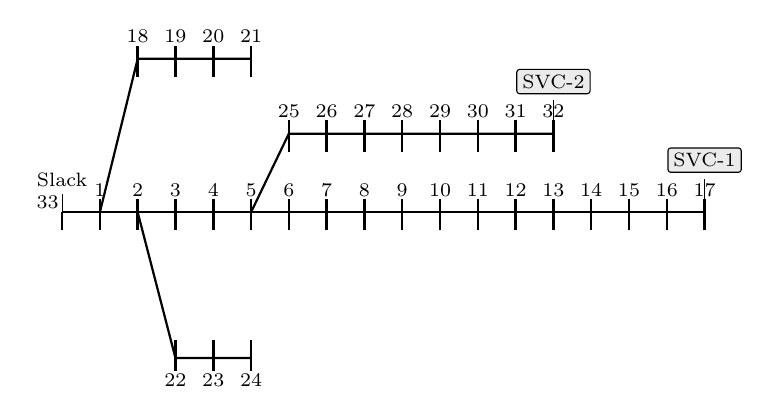
\begin{tikzpicture}[
        x=0.48cm,
        y=0.95cm,
        busbar/.style={line width=0.9pt},
        buslabel/.style={font=\scriptsize, inner sep=1pt, fill=white},
        svc/.style={draw, rounded corners=1pt, fill=black!8, inner sep=2pt, font=\scriptsize},
        feeder/.style={thick}
    ]
        % Slack bus and main feeder
        \coordinate (b33) at (0,0);
        \draw[busbar] ($(b33)+(0,-0.24)$) -- ($(b33)+(0,0.24)$);
        \node[buslabel, above left=0mm and 0mm of b33] {33};
        \node[above=2mm of b33, font=\scriptsize] {Slack};

        \foreach \n/\x in {1/1,2/2,3/3,4/4,5/5,6/6,7/7,8/8,9/9,10/10,11/11,12/12,13/13,14/14,15/15,16/16,17/17} {
            \coordinate (b\n) at (\x,0);
            \draw[busbar] ($(b\n)+(0,-0.24)$) -- ($(b\n)+(0,0.24)$);
            \node[buslabel, above=1.6mm of b\n] {\n};
        }

        % Upper laterals from buses 1 and 5
        \foreach \n/\x in {18/2,19/3,20/4,21/5} {
            \coordinate (b\n) at (\x,2.05);
            \draw[busbar] ($(b\n)+(0,-0.24)$) -- ($(b\n)+(0,0.24)$);
            \node[buslabel, above=1.6mm of b\n] {\n};
        }
        \foreach \n/\x in {25/6,26/7,27/8,28/9,29/10,30/11,31/12,32/13} {
            \coordinate (b\n) at (\x,1.05);
            \draw[busbar] ($(b\n)+(0,-0.24)$) -- ($(b\n)+(0,0.24)$);
            \node[buslabel, above=1.6mm of b\n] {\n};
        }

        % Lower lateral from bus 2
        \foreach \n/\x in {22/3,23/4,24/5} {
            \coordinate (b\n) at (\x,-1.95);
            \draw[busbar] ($(b\n)+(0,-0.24)$) -- ($(b\n)+(0,0.24)$);
            \node[buslabel, below=1.6mm of b\n] {\n};
        }

        % Feeder connections
        
        \draw[feeder] (b1) -- (b18) -- (b21);
        \draw[feeder] (b2) -- (b22) -- (b24);
        \draw[feeder] (b5) -- (b25) -- (b32);
        \draw[feeder] (b1) -- (b17);
        \draw[feeder] (b33) -- (b1);

        % Controlled SVC markers in shifted numbering
        \node[svc, above=5mm of b17] {SVC-1};
        \draw[thin] (b17) -- ++(0,0.45);
        \node[svc, above=5mm of b32] {SVC-2};
        \draw[thin] (b32) -- ++(0,0.45);
    \end{tikzpicture}%
    }
    \caption{Single-line diagram of the adopted IEEE 33-bus system.}
    \label{fig:ieee33_singleline}
\end{figure}



For the 33-bus distribution system,
$V_{\mathrm{LL,nom}} = 12.66$~kV, the electrical parameters and reactive-power operating ranges of the two
controlled compensators adopted are summarized in
Table~\ref{tab:svc_parameters}

\begin{table}[htbp]
\centering
\caption{Parameters of the static VAr compensators}
\label{tab:svc_parameters}
\begin{threeparttable}
\footnotesize
\renewcommand{\arraystretch}{1.25}
\setlength{\tabcolsep}{3pt}
\begin{tabular}{@{}p{0.50\columnwidth}>{\centering\arraybackslash}p{0.20\columnwidth}>{\centering\arraybackslash}p{0.20\columnwidth}@{}}
\toprule
\textbf{Parameter} & \textbf{Bus 17} & \textbf{Bus 32} \\
\midrule
Bus number & 17 & 32 \\
Firing angles $\alpha_{j,\ell}$ (deg) & 90.00--180.00 & 90.00--180.00 \\
Control variables & $\alpha_{17,ab}$, $\alpha_{17,bc}$, $\alpha_{17,ca}$ & $\alpha_{32,ab}$, $\alpha_{32,bc}$, $\alpha_{32,ca}$ \\
\midrule
\multicolumn{3}{@{}l}{\textit{Thyristor-controlled reactor (TCR) --- per delta branch}} \\
\midrule
Inductance $L_j$ (mH) & 2.500 & 2.650 \\
Resistance $R_j$ ($\Omega$) & 0.001 & 0.001 \\
Reactance $X_{L,j}=\omega L_j$ ($\Omega$) & 0.942 & 0.999 \\
Reactance $X_{L,j}$ (pu)\tnote{a} & 0.00588 & 0.00623 \\
\midrule
\multicolumn{3}{@{}l}{\textit{Capacitor bank --- per delta branch}} \\
\midrule
Capacitance $C_j$ ($\mu$F) & 2652.6 & 2652.6 \\
Reactance $X_{C,j}=1/\omega C_j$ ($\Omega$) & 1.000 & 1.000 \\
Reactance $X_{C,j}$ (pu)\tnote{a} & 0.00624 & 0.00624 \\
\midrule
\multicolumn{3}{@{}l}{\textit{Three-phase reactive-power range from harmonic power flow}} \\
\midrule
$Q_{\mathrm{SVC},j}^{\min}$ (kVAr)\tnote{b} & $-231.4$ & $-117.1$ \\
$Q_{\mathrm{SVC},j}^{\max}$ (kVAr)\tnote{c} & $+3210.8$ & $+3065.1$ \\
Control range $\Delta Q_{\mathrm{SVC},j}$ (kVAr) & $3442.2$ & $3182.2$ \\
\bottomrule
\end{tabular}

\begin{tablenotes}
\scriptsize
\item[a] Per-unit values on the system base: $S_b=1$ MVA, $V_b=12.66$ kV, and $Z_b=V_b^2/S_b=160.28\,\Omega$.
\item[b] $Q_{\mathrm{SVC},j}^{\min}$ corresponds to $\alpha_{j,\ell}=90.00^\circ$ in all delta branches, i.e., full TCR conduction; the negative sign indicates inductive operation.
\item[c] $Q_{\mathrm{SVC},j}^{\max}$ corresponds to $\alpha_{j,\ell}=180.00^\circ$ in all delta branches, i.e., complete blocking of the TCR branch; the positive sign indicates capacitive operation.
\end{tablenotes}
\end{threeparttable}
\end{table}



% -------------------------------------------------------------------------



Because the analyzed feeder may operate under balanced or unbalanced loading
conditions, the load curve is represented in phase-dependent form. At each
operating point $k$, the active and reactive demands at bus $i$ and phase
$\phi$ are scaled as\vspace{-1em}

\begin{align}
    P_{i,\phi,k} &= \lambda_{i,\phi,k} P_{i,\phi}^{0}, \\
    Q_{i,\phi,k} &= \lambda_{i,\phi,k} Q_{i,\phi}^{0},
    \label{eq:phase_load_scaling}
\end{align}

\noindent where $P_{i,\phi}^{0}$ and $Q_{i,\phi}^{0}$ are the nominal phase
loads and $\lambda_{i,\phi,k}$ is the load multiplier assigned to that
specific bus, phase, and operating point. The complete load trajectory is described by the set\vspace{-1em}

\begin{equation}
    \boldsymbol{\Lambda} =
    \left[\lambda_{i,\phi,k}\right]_{i\in\mathcal{B},\,\phi\in\Phi,\,k=1,\ldots,N_p},
    \label{eq:phase_load_curve}
\end{equation}

\noindent rather than by a single scalar load multiplier. This representation
allows each phase to follow a different trajectory and is therefore suitable
for unbalanced load-growth or daily-load scenarios. The conventional balanced
load curve is recovered as a particular case by imposing
$\lambda_{i,a,k}=\lambda_{i,b,k}=\lambda_{i,c,k}=\lambda_k$ for all buses
and operating points. In the results, the horizontal loading variable denotes
the common factor $\lambda_k$ in balanced studies and the reference loading
level associated with $\boldsymbol{\Lambda}$ in unbalanced studies.



\subsection{Balanced Loading Condition}
\label{subsec:balanced_results}

In this scenario, identical active and reactive powers are assigned to the three phases at each load bus. Therefore, the optimized firing angles are expected to be equal or nearly equal, allowing the proposed formulation to be assessed under conventional balanced operating conditions.

Fig.~\ref{fig:balanced_voltage_all_buses} shows the fundamental-frequency voltage magnitudes as a function of the load multiplier $\lambda_k$. As expected in a radial feeder, downstream buses experience larger voltage drops as loading increases. Nevertheless, the optimized SVC operation maintains bus voltages within the prescribed limits over the feasible loading range. The three phase trajectories overlap, as expected under balanced conditions.

\begin{figure}[!h]
    \centering
    \stdplot[scale=0.4]{caso equilibrado/figura_02.pdf}
      {Load multiplier, $\lambda$}
      {Voltage magnitude, $|V^{(1)}|$ [pu]}
    \caption{Fundamental-voltage magnitude as a function of the load multiplier for all buses.}
    \label{fig:balanced_voltage_all_buses}
\end{figure}

The corresponding voltage profiles along the feeder are presented in Fig.~\ref{fig:balanced_voltage_profiles} for selected load multipliers. The increasing voltage drop toward the feeder end is evident, while the optimized compensators provide the required voltage support at the controlled buses.

\begin{figure}[!h]
    \centering
    \stdplot[scale=0.4]{caso equilibrado/figura_08.pdf}
      {Bus index, $i$}
      {Voltage magnitude, $|V^{(1)}|$ [pu]}
    \caption{Fundamental-voltage profiles for different load multipliers.}
    \label{fig:balanced_voltage_profiles}
\end{figure}

Fig.~\ref{fig:balanced_voltage_bus17}  details the voltage magnitudes at bus 17. The overlapping phase trajectories confirm the balanced response, while the voltage magnitudes remain within the prescribed operating limits throughout the analyzed loading range.

\begin{figure}[!h]
    \centering
    \stdplot[scale=0.45]{caso equilibrado/figura_06.pdf}
      {Load multiplier, $\lambda$}
      {Voltage magnitude, $|V^{(1)}|$ [pu]}
    \caption{Voltage magnitude at the controlled SVC bus 17.}
    \label{fig:balanced_voltage_bus17}
\end{figure}



The harmonic performance is evaluated through the voltage total harmonic distortion. Fig.~\ref{fig:balanced_thdv_all_buses} shows that $\mathrm{THD}_V$ remains below the adopted 8.00\% IEC compatibility level throughout the simulated loading range. Differences among buses arise from the interaction between the harmonic currents injected by the SVCs and the harmonic impedance of the feeder.

\begin{figure}[!h]
    \centering
    \stdplot[scale=0.4]{caso equilibrado/figura_03.pdf}
      {Load multiplier, $\lambda$}
      {Voltage THD, $\mathrm{THD}_V$ [\%]}
    \caption{Voltage THD as a function of the load multiplier for all buses.}
    \label{fig:balanced_thdv_all_buses}
\end{figure}

The phase $\mathrm{THD}_V$ at bus 17 is detailed in Fig.~\ref{fig:balanced_thdv_bus17}. The nearly coincident phase trajectories confirm the symmetrical harmonic response under balanced loading. Moreover, distortion remains below the imposed limit at both locations, indicating that voltage support is achieved without violating the harmonic constraint.

\begin{figure}[!h]
    \centering
    \stdplot[scale=0.45]{caso equilibrado/figura_05.pdf}
      {Load multiplier, $\lambda$}
      {Voltage THD, $\mathrm{THD}_V$ [\%]}
    \caption{Voltage THD at bus 17 as a function of the load multiplier (balanced case).}
    \label{fig:balanced_thdv_bus17}
\end{figure}



Finally, Fig.~\ref{fig:balanced_firing_angles} presents the optimized SVC firing angles. At low loading levels, the angles remain close to $90.00^\circ$, resulting in stronger TCR conduction. 

\begin{figure}[!h]
    \centering
    \stdplot[scale=0.4]{caso equilibrado/figura_01.pdf}
      {Load multiplier, $\lambda$}
      {Firing angle, $\alpha$ [deg]}
    \caption{Firing angles of the controlled SVCs as a function of the load multiplier (balanced case).}
    \label{fig:balanced_firing_angles}
\end{figure}

As loading increases, the angles approach $180.00^\circ$, reducing reactor conduction and increasing the net capacitive effect. This behavior is consistent with the increasing reactive power support required to maintain voltage levels under heavier loading conditions.

% -------------------------------------------------------------------------

\subsection{Three-Phase Unbalanced Loading Condition}
\label{subsec:unbalanced_results}

The unbalanced operating condition is evaluated over a 24-hour trajectory with independent load multipliers for phases $a$, $b$, and $c$, as defined by the phase-dependent load curve $\boldsymbol{\Lambda}$ in~\eqref{eq:phase_load_curve}. The voltage-unbalance limit is set to $\mathrm{VUF}^{\max}=1.00\%$, providing a more restrictive condition than the general numerical settings and testing the ability of the proposed formulation to actively reduce the negative-sequence component through independent branch-wise firing angles. No external harmonic sources are considered; thus, the harmonic distortion results exclusively from the two SVC compensators.

Fig.~\ref{fig:unbalanced_loading_profiles} presents the daily loading profiles applied to phases $a$, $b$, and $c$ at both controlled buses (17 and 32). The different temporal variations among phases create time-varying unbalance conditions, allowing the evaluation of the adaptive compensation provided by the proposed control strategy.

\begin{figure}[!h]
    \centering
    \stdplot[scale=0.38]{caso desequilibrado/figura_01.pdf}
      {Time, $t$ [h]}
      {Phase load multiplier, $\lambda_{\phi}$}
    \caption{Daily phase load multipliers used in the unbalanced case.}
    \label{fig:unbalanced_loading_profiles}
\end{figure}

The voltage-balancing performance is first assessed through the VUF defined in~\eqref{eq:vuf}. Fig.~\ref{fig:unbalanced_vuf_bus17} compares its values at bus 17 with and without SVC compensation. The optimized controller maintains the VUF below the imposed 1.00\% limit, whereas the uncompensated case exhibits higher unbalance. This improvement results from the independent adjustment of the delta-branch susceptances, as defined in~\eqref{eq:svc_susceptance}, which enables the controller to redistribute reactive compensation according to the phase-dependent loading conditions.

\begin{figure}[!h]
    \centering
    \stdplot[scale=0.38]{caso desequilibrado/figura_02.pdf}
      {Time, $t$ [h]}
      {Voltage unbalance factor, VUF [\%]}
    \caption{VUF at bus 17 without SVC and with optimized SVC operation.}
    \label{fig:unbalanced_vuf_bus17}
\end{figure}

The corresponding phase-voltage magnitudes are shown in Fig.~\ref{fig:unbalanced_phase_voltage_bus17}. The optimized operation reduces the separation among phases while maintaining the voltages within the prescribed operating range, demonstrating that phase balancing is achieved without compromising voltage regulation.

\begin{figure}[!h]
    \centering
    \stdplot[scale=0.38]{caso desequilibrado/figura_04.pdf}
      {Time, $t$ [h]}
      {Voltage magnitude, $|V^{(1)}|$ [pu]}
    \caption{Phase-voltage magnitudes at bus 17 in the unbalanced case without SVC and with optimized SVC operation.}
    \label{fig:unbalanced_phase_voltage_bus17}
\end{figure}

The control mechanism responsible for these improvements is illustrated in Fig.~\ref{fig:unbalanced_firing_angles_bus17}. Unlike the balanced case, the optimized firing angles differ among phases, reflecting the independent adjustment of the delta branches to provide the required asymmetric reactive compensation.

\begin{figure}[!h]
    \centering
    \stdplot[scale=0.38]{caso desequilibrado/figura_05.pdf}
      {Time, $t$ [h]}
      {Firing angle, $\alpha$ [deg]}
    \caption{Firing angles of the SVC at bus 17 in the unbalanced case.}
    \label{fig:unbalanced_firing_angles_bus17}
\end{figure}

Fig.~\ref{fig:unbalanced_phase_voltage_deviation_bus17} further illustrates the voltage-regulation performance. The optimized response keeps phase-voltage deviations closer to zero, indicating improved voltage regulation and reduced dispersion throughout the daily loading trajectory. This behavior is also reflected in the voltage envelope shown in Fig.~\ref{fig:unbalanced_voltage_envelope_bus17}, where the optimized operation produces a narrower voltage range within the admissible limits.

\begin{figure}[!h]
    \centering
    \stdthreephaseplot[scale=0.38]{caso desequilibrado/figura_07.pdf}
    \caption{Phase-voltage deviations at bus 17 in the unbalanced case without SVC and with optimized SVC operation.}
    \label{fig:unbalanced_phase_voltage_deviation_bus17}
\end{figure}

\begin{figure}[!h]
    \centering
    \stdplot[scale=0.38]{caso desequilibrado/figura_09.pdf}
      {Time, $t$ [h]}
      {Voltage magnitude, $|V^{(1)}|$ [pu]}
    \caption{Voltage envelope at bus 17 in the unbalanced case.}
    \label{fig:unbalanced_voltage_envelope_bus17}
\end{figure}

The harmonic impact of the optimized operation is evaluated in Figs.~\ref{fig:unbalanced_thdv_envelope_bus17} and~\ref{fig:unbalanced_thdv_phase_bus17}. Since no external harmonic sources are included, the resulting $\mathrm{THD}_V$ is associated with the harmonic currents injected by the two SVCs and their interaction with the feeder harmonic admittance. Both the voltage-distortion envelope and the individual phase values remain below the adopted 8.00\% limit, indicating that the VUF reduction does not result in excessive harmonic distortion.

\begin{figure}[!h]
    \centering
    \stdplot[scale=0.38]{caso desequilibrado/figura_10.pdf}
      {Time, $t$ [h]}
      {Voltage THD, $\mathrm{THD}_V$ [\%]}
    \caption{Voltage-THD envelope at bus 17 in the unbalanced case.}
    \label{fig:unbalanced_thdv_envelope_bus17}
\end{figure}

\begin{figure}[!h]
    \centering
    \stdplot[scale=0.38]{caso desequilibrado/figura_11.pdf}
      {Time, $t$ [h]}
      {Voltage THD, $\mathrm{THD}_V$ [\%]}
    \caption{Phase voltage THD at bus 17 in the optimized unbalanced case.}
    \label{fig:unbalanced_thdv_phase_bus17}
\end{figure}

The same analysis is performed at bus 32, the second controlled SVC location. To avoid repeating the previous discussion, the following results focus on the main indicators of phase balancing, voltage regulation, and harmonic performance.

Fig.~\ref{fig:unbalanced_vuf_bus32} shows that the optimized controller also maintains the VUF below the imposed 1.00\% limit at bus 32. The corresponding firing angles, presented in Fig.~\ref{fig:unbalanced_firing_angles_bus32}, exhibit phase-dependent trajectories, confirming that the three delta branches are independently adjusted to accommodate the unbalanced loading conditions.

\begin{figure}[!h]
    \centering
    \stdplot[scale=0.38]{caso desequilibrado/barra 32/figura_11.pdf}
      {Time, $t$ [h]}
      {Voltage unbalance factor, VUF [\%]}
    \caption{Voltage unbalance factor at bus 32 in the unbalanced case without SVC and with optimized SVC operation.}
    \label{fig:unbalanced_vuf_bus32}
\end{figure}

\begin{figure}[!h]
    \centering
    \stdplot[scale=0.38]{caso desequilibrado/barra 32/figura_08.pdf}
      {Time, $t$ [h]}
      {Firing angle, $\alpha$ [deg]}
    \caption{Firing angles of the controlled SVC at bus 32 in the unbalanced case.}
    \label{fig:unbalanced_firing_angles_bus32}
\end{figure}

The voltage envelope at bus 32, shown in Fig.~\ref{fig:unbalanced_voltage_envelope_bus32}, confirms that the reduction in phase unbalance is accompanied by improved voltage regulation. 

\begin{figure}[!h]
    \centering
    \stdplot[scale=0.38]{caso desequilibrado/barra 32/figura_04.pdf}
      {Time, $t$ [h]}
      {Voltage magnitude, $|V^{(1)}|$ [pu]}
    \caption{Voltage envelope at bus 32 in the unbalanced case.}
    \label{fig:unbalanced_voltage_envelope_bus32}
\end{figure}






\color{black}
\subsection{Balanced-Loading Tests on the IEEE 123-Node Test Feeder}
\label{subsec:ieee123_results}

The large-scale assessment uses the standard IEEE 123-node test feeder defined
by Kersting~\cite{Kersting2001RadialFeeders}, imported from the corresponding
test-case implementation distributed with OpenDSS by EPRI~\cite{EPRIOpenDSSTestCases}.
Thus, the underlying feeder is the original IEEE benchmark circuit rather than
a different 123-bus network; the FC--TCR devices and the harmonic-domain model
described in this work are added to this base system. After import, the network
representation contains 132 physical buses, 278 active bus--phase nodes, 126
lines, 91 loads, four capacitor banks, and bus 150 as the slack bus. The
retained harmonic set is
$\mathcal{H}=\{1,3,5,7,11,13\}$, resulting in 3336 simultaneous rectangular
state variables. At every operating point, all harmonic voltages are solved
simultaneously by the Harmonic Three-Phase Current Injection Method (HTPCIM)
inside the reduced-space state solution, with a current-mismatch tolerance of
$10^{-7}$~pu in this experiment. External load-harmonic sources are disabled;
therefore, the reported distortion is produced by the FC--TCR devices and its
propagation through the network.

\subsubsection{SVC location screening}

The SVC locations were defined before the loading sweep through a two-stage
sensitivity-and-complementarity screening. Sensitivity indices are widely
used to identify buses at which a shunt compensator has strong influence on
the network voltages~\cite{JainDahiya2016SVCPlacement}. In harmonic studies,
normalized sensitivity measures likewise provide a computationally efficient
first screening of candidate locations before the selected alternatives are
tested with the complete nonlinear model~\cite{AuMilanovic2007HarmonicPlacement}.
When more than one dynamic reactive-power device is installed, location should
also account for the controllability supplied by the complete set, instead of
ranking every device independently~\cite{Qi2017DynamicVarPlacement}. Motivated
by these three principles, this work combines individual control authority
with a nonredundancy measure tailored to the multiphase harmonic response of
the IEEE 123-node feeder. The particular weighted score, sensitivity
fingerprint, cosine-based complementarity measure, and numerical weights
introduced below are formulations proposed in this work.

The eligible set contained 64
three-phase buses. The slack and gauge buses, open points, internal regulator
buses, and the immediate slack-neighborhood bus were excluded because they do
not represent admissible distribution-level installation points. At each
remaining bus, independent normalized incremental shunt-susceptance
perturbations were applied to phases A, B, and C around the solved base case.
The resulting first-order responses were used only as controllability indices;
the final simulations still employ the complete nonlinear FC--TCR model.

For the fundamental component, the voltage response to each perturbation was
obtained from the solved fundamental Jacobian. For each retained
nonfundamental harmonic $h$, the first-order voltage response to a small
shunt-susceptance perturbation was obtained by solving the frequency-dependent
linear sensitivity equation
$\bm{Y}_{h}(\partial\bm{V}_{h}/\partial b)
=-\partial\bm{I}_{h}/\partial b$. This calculation was used only for location
screening; the final simulations were performed using the complete nonlinear
FC--TCR model. The three phase responses were aggregated by their
root-mean-square values. Each raw indicator was then min--max normalized over
the candidate set, and the individual score of candidate bus $i$ was defined
as

\begin{equation}
\begin{split}
S_i={}&0.45\widehat{s}_{\mathrm{THD,rms},i}
 +0.20\widehat{s}_{\mathrm{THD,crit},i}
 +0.15\widehat{s}_{V,\mathrm{rms},i}\\
 &+0.10\widehat{s}_{\mathrm{VUF,rms},i}
 +0.10\widehat{\mathrm{THD}}_{\mathrm{local},i},
\end{split}
\label{eq:svc_location_individual_score}
\end{equation}

where hats denote quantities normalized to $[0,1]$ across the 64 candidates.
The first term measures the RMS sensitivity of feeder-wide THD; the second
measures the THD sensitivity at the most distorted bus--phase node; the third
and fourth measure the RMS sensitivities of fundamental-voltage magnitude and
VUF, respectively; and the last term represents the pre-control local THD.
Thus, the ranking favors buses that influence both the critical location and
the network as a whole, rather than selecting a location solely from its local
voltage or distortion.

The weights in~\eqref{eq:svc_location_individual_score} express the priorities
of the present experiment and sum to unity. Feeder-wide THD sensitivity
receives the largest weight, 0.45, because a device that improves only its
installation bus can leave distortion at downstream or lateral nodes
unaffected. The critical-node term receives 0.20 so that a good network-wide
average cannot conceal a weak action at the most distorted bus--phase node.
Fundamental-voltage sensitivity receives 0.15 because voltage regulation is a
primary function of the SVC, even though the base-case screening is dominated
by harmonic distortion. VUF sensitivity receives 0.10 to retain the benefit
of the three independently controlled phases for unbalance mitigation. The
remaining 0.10 assigned to local pre-control THD favors electrically relevant
regions without allowing local severity alone to determine the location.
These coefficients are engineering priorities for screening, not universal
physical constants; consequently, the selected buses are subsequently
verified by the full nonlinear FC--TCR simulations.

Selecting the two largest individual scores could place both devices at
electrically adjacent locations with nearly identical effects. To penalize
this redundancy, each bus was also represented by a fingerprint $\bm f_i$
formed by stacking its phase-dependent THD sensitivities at all valid
bus--phase nodes. For every pair $(i,j)$, redundancy and complementarity were
computed as

\begin{equation}
\rho_{ij}=\frac{|\bm f_i^{\mathsf T}\bm f_j|}
{\|\bm f_i\|_2\|\bm f_j\|_2},\qquad
C_{ij}=\sqrt{1-\rho_{ij}^{2}}.
\label{eq:svc_location_complementarity}
\end{equation}

Accordingly, $C_{ij}=0$ indicates collinear, redundant responses, whereas
$C_{ij}=1$ indicates orthogonal sensitivity patterns. Pair quality and the
final pair score were calculated from

\begin{equation}
\begin{aligned}
Q_{ij}&=0.70\,\operatorname{mean}(S_i,S_j)
       +0.30\,\min(S_i,S_j),\\
P_{ij}&=0.65Q_{ij}+0.35C_{ij}.
\end{aligned}
\label{eq:svc_location_pair_score}
\end{equation}

The mean-score contribution in $Q_{ij}$ rewards the total control authority
of the pair, whereas the minimum-score contribution prevents one strong bus
from compensating numerically for one weak bus. The 0.70/0.30 split therefore
retains overall effectiveness as the main criterion while explicitly
protecting the weaker device location. In $P_{ij}$, individual pair quality
remains dominant with weight 0.65, and 0.35 is reserved for complementarity.
This choice rejects strongly redundant pairs without selecting two mutually
different but individually ineffective buses. As with the individual score,
these values define a reproducible design preference rather than a generally
optimal weighting for every feeder.

In the base case, the critical node was phase C of bus 83, with a THD of
23.49\%. Bus 83 ranked first among the individual candidates
($S_{83}=1.00$ after rounding), while bus 95 ranked seventh
($S_{95}=0.68$). Their complementarity was $C_{83,95}=0.64$, resulting in a
pair score of $P_{83,95}=0.74$. Hence, bus 83 provides strong authority over
the critical distortion region, while bus 95 contributes a sufficiently
distinct feeder-wide response. This balance between individual influence and
nonredundancy motivated the use of buses 83 and 95 in the two-device study.

For the four-device computational experiment, buses 83 and 95 were kept fixed
and every candidate pair of additional locations was evaluated. The set
quality retained the same $0.70$ mean-score and $0.30$ minimum-score terms,
now applied to all four buses. Set complementarity was conservatively defined
as the minimum $C_{ij}$ among the six pairs in the four-bus set, so that one
nearly duplicated device could not be hidden by a high average. This condition
is a weakest-link criterion: every added device must contribute a sufficiently
distinct response relative to every device already selected. It is important
because bus 82 had a high individual score of 0.92 but was almost
redundant with bus 83 ($C_{83,82}=0.04$). The conditioned screening therefore
selected buses 72 and 300 as the additional locations. Their individual scores
were 0.54 and 0.52, respectively; for the complete set
$\{83,95,72,300\}$, the minimum pairwise complementarity was 0.39 and the
maximum was 0.82. This screening is a reproducible engineering criterion for
device placement, but it is not presented as a proof of globally optimal
siting, which would require solving and comparing the complete nonlinear
placement-and-control problem.

Two FC--TCR SVCs are installed at buses 83 and 95. Two electrically equivalent
connection alternatives are evaluated: grounded wye and delta. In both cases,
each device combines a 300-kVAr fixed capacitor with a 400-kVAr
thyristor-controlled reactor, giving an approximate net range from $-100$ to
$+300$~kVAr at nominal voltage. In grounded wye, the three controlled elements
are connected from phases A, B, and C to ground. In delta, the controlled
elements form branches $ab$, $bc$, and $ca$. Thus, the six-dimensional reduced
control vector can be written generically as

\begin{equation}
 \begin{aligned}
 \bm{\alpha}={}&[\alpha_{83,1},\alpha_{83,2},\alpha_{83,3},\\
 &\alpha_{95,1},\alpha_{95,2},\alpha_{95,3}]^{\top},\\
 &90.00^\circ\leq\alpha_{j,k}\leq180.00^\circ,
 \end{aligned}
 \label{eq:ieee123_control_vector}
\end{equation}
where $k\in\{A,B,C\}$ for grounded wye and
$k\in\{ab,bc,ca\}$ for delta.

The normalized outer variables are $z_{j,k}=\alpha_{j,k}/90$, with
$1\leq z_{j,k}\leq2$. For every trial control, the 3336 state variables
are recovered implicitly from the HTPCIM equations, and the reduced
derivatives are evaluated from
$d\bm{y}/d\bm{z}=-\bm{F}_{\bm{y}}^{-1}\bm{F}_{\bm{z}}$.
Table~\ref{tab:svc_parameters123_current} gives the parameters used for both
devices under each connection.

\begin{table}[!t]
\centering
\caption{Equivalent FC--TCR parameters for each connection in the IEEE 123-node feeder}
\label{tab:svc_parameters123_current}
\setlength{\tabcolsep}{4pt}
\renewcommand{\arraystretch}{1.08}
\begin{tabular}{@{}lcc@{}}
\toprule
Parameter & Grounded wye & Delta \\
\midrule
Controlled elements & A--N, B--N, C--N & $ab$, $bc$, $ca$ \\
Nominal line voltage (kV) & 4.16 & 4.16 \\
FC rating (kVAr) & 300 & 300 \\
TCR rating (kVAr) & 400 & 400 \\
Net nominal range (kVAr) & $-100$ to $+300$ & $-100$ to $+300$ \\
$C$ per element ($\mu$F) & 45.984 & 15.328 \\
$L$ per element (mH) & 114.761 & 344.284 \\
$R$ per element ($\Omega$) & 0.1298 & 0.3894 \\
Firing-angle interval (deg) & 90.00--180.00 & 90.00--180.00 \\
\bottomrule
\end{tabular}
\end{table}

The parameter conversion follows directly from the voltage applied to each
element. A grounded-wye element is subjected to phase-to-neutral voltage,
whereas a delta element is subjected to line-to-line voltage. Consequently,
for the same total three-phase reactive-power rating,
$C_{\Delta}=C_{Y}/3$ and $L_{\Delta}=3L_{Y}$; the resistance is also multiplied
by three to preserve the adopted $X/R$ ratio. This conversion changes the
connection topology without changing the nominal FC and TCR ratings.

The connections provide different sequence-current paths. Grounded wye permits
phase-to-ground current exchange and therefore direct phase-wise and
zero-sequence voltage support. Delta has no external neutral, and its branch
currents are transformed into line currents through the delta incidence
relation in~\eqref{eq:delta_incidence}. Ideally, triplen and zero-sequence
components circulate inside the closed delta or cancel at its terminals. This
property can reduce harmonic current transfer to the feeder, but it also
removes part of the independent phase-to-ground support available from the
grounded-wye connection.

\subsubsection{Balanced loading trajectory and optimization settings}

The loading experiment contains 24 equally spaced operating points from
$\lambda=1.00$ to $\lambda=2.00$. The same multiplier is applied to phases A,
B, and C at each point. Thus, the trajectory is balanced with respect to its
phase multipliers, although the original IEEE 123 feeder remains structurally
unbalanced because its phase connections, spatial load distribution, and
network topology are preserved. The points represent a loading sweep rather
than chronological hours or a closed-loop dynamic simulation. The solution of
one point is used as the warm start for the next point.

The objective is
\begin{equation}
 J=1000J_{\mathrm{dev}}+1000J_{\mathrm{neg}}+200J_{\mathrm{imb}},
 \label{eq:ieee123_balanced_objective}
\end{equation}
and is evaluated at the two controlled buses. The imposed limits are
$0.95\leq|V^{(1)}|\leq1.05$~pu, $\mathrm{VUF}\leq2.00\%$, and
$\mathrm{THD}\leq7.10\%$, in addition to the firing-angle bounds. These are
the numerical limits of this benchmark and should not be interpreted as a
general regulatory-compliance assessment.

In the following discussion, \emph{optimization-feasible} means that all the
inequality limits above are satisfied. A point classified as infeasible by the
optimizer is nevertheless retained as a valid electrically solved operating
point whenever the HTPCIM power flow converges. Such a point is acceptable for
electrical comparison and continuation of the loading sweep, although it does
not comply with one or more imposed benchmark limits. Hence, optimization
infeasibility must not be confused with failure of the electrical solution.

\subsubsection{Results of the 24-point sweep}

All 24 grounded-wye points and all 24 delta points converge electrically and
are therefore valid operating points for the comparison. Under the optimization
limits, grounded wye is feasible at 22 points, through $\lambda=1.91$, whereas
delta is feasible at 21 points, through $\lambda=1.87$. The remaining points
are classified as optimization-infeasible only because at least one controlled
phase falls below 0.95~pu. Their converged HTPCIM solutions remain electrically
valid and are included in every curve and aggregate statistic.

Fig.~\ref{fig:ieee123_phase_voltages_connections} presents the fundamental
voltage of every controlled phase instead of a minimum--maximum envelope. At
bus 83, grounded wye provides slightly better phase-A support at high loading,
while delta produces a higher phase-B voltage. The same tendency is visible at
bus 95. The worst voltage is 0.94~pu for both connections when rounded to two
decimal places, but the unrounded delta minimum is lower and crosses the
0.95-pu benchmark one loading point earlier. This result is consistent with
the direct phase-to-ground current path of grounded wye and the absence of an
external zero-sequence path in delta.

\begin{figure*}[!t]
    \centering
    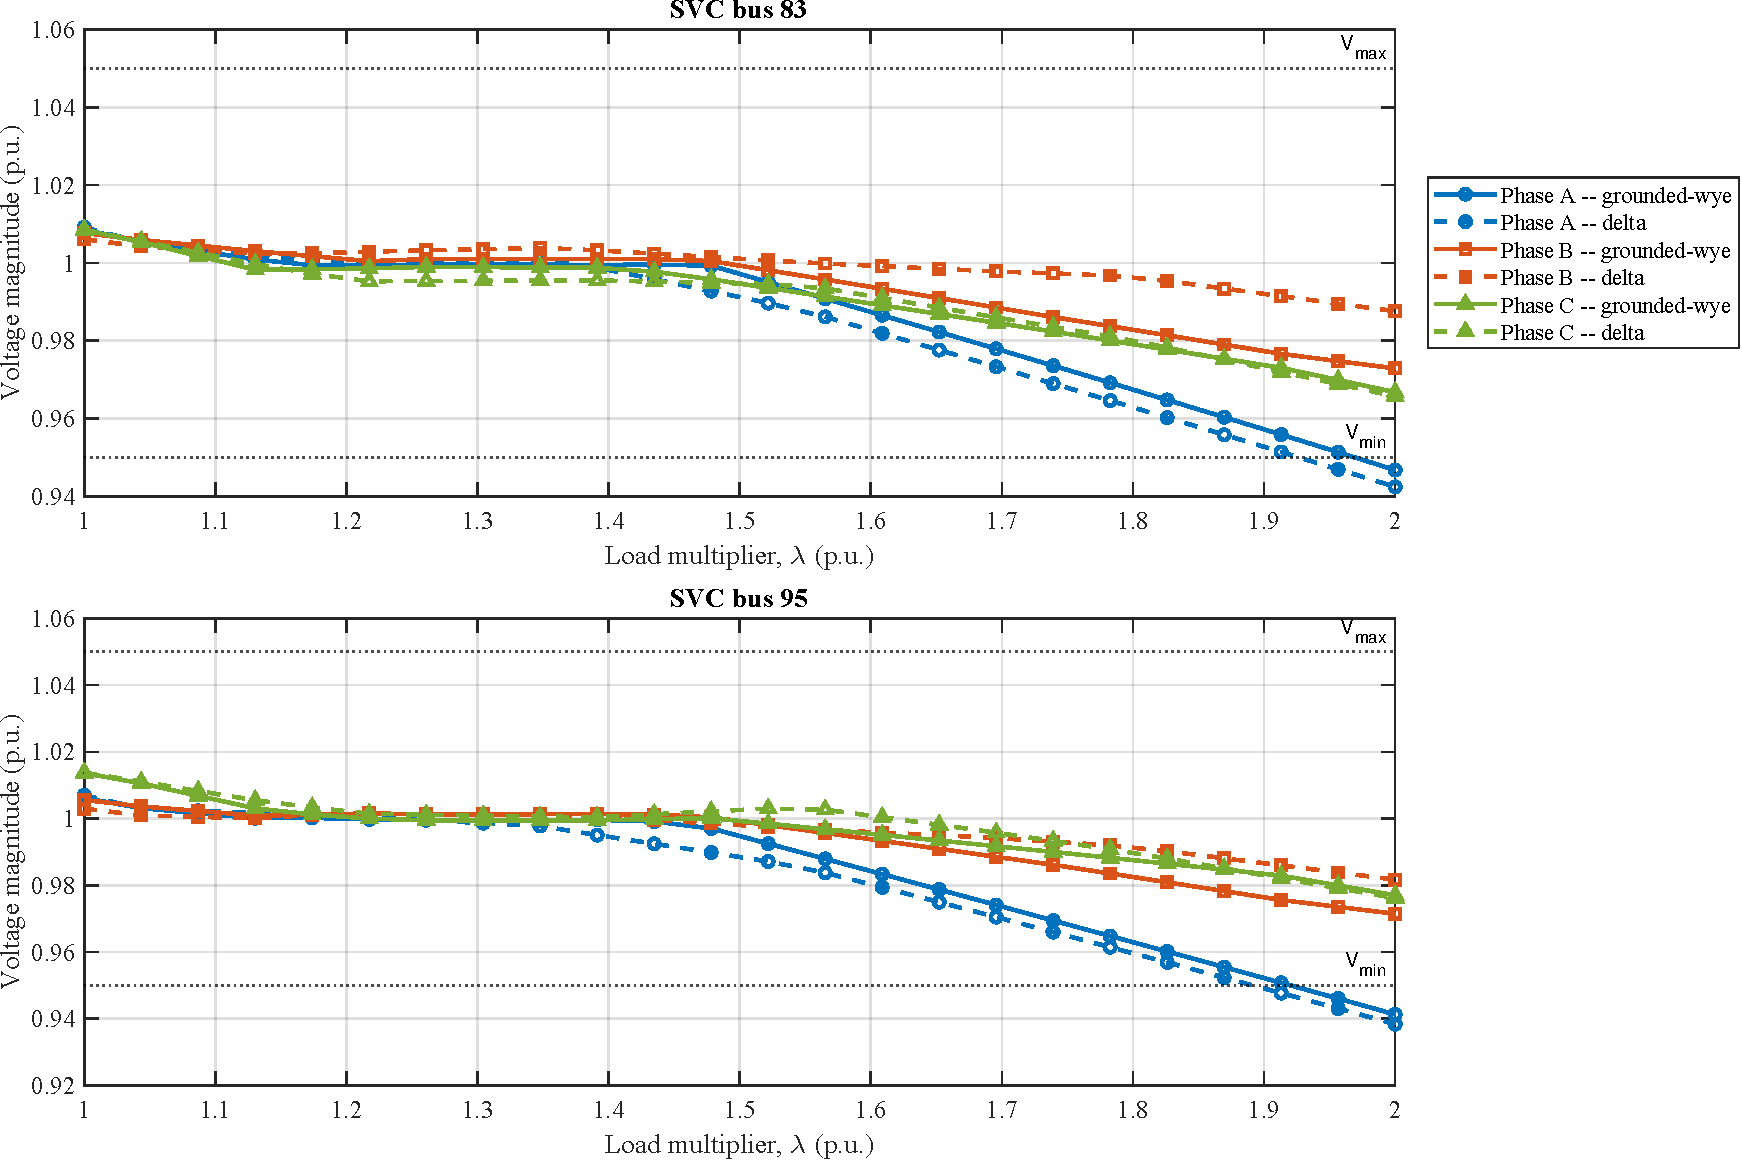
\includegraphics[width=0.96\textwidth]{figuras_ieee123_equilibrado/controlled_phase_voltages_wye_delta.pdf}
    \caption{Fundamental-frequency phase voltages at buses 83 and 95 for
    grounded-wye and delta SVC connections. Solid curves denote grounded wye,
    and dashed curves denote delta. All points shown are converged electrical
    solutions; points outside the 0.95--1.05-pu band are classified only as
    infeasible with respect to the optimization constraints.}
    \label{fig:ieee123_phase_voltages_connections}
\end{figure*}

\begin{table}[!t]
\centering
\caption{Comparison over the balanced 24-point IEEE 123-node loading sweep}
\label{tab:ieee123_24h_summary}
\setlength{\tabcolsep}{4pt}
\renewcommand{\arraystretch}{1.08}
\begin{tabular}{@{}lcc@{}}
\toprule
Quantity & Grounded wye & Delta \\
\midrule
Electrically converged points & 24/24 & 24/24 \\
Optimization-feasible points & 22/24 & 21/24 \\
Last feasible load multiplier & 1.91 & 1.87 \\
Minimum controlled voltage (pu) & 0.94 & 0.94 \\
Mean pointwise maximum VUF (\%) & 1.36 & 1.20 \\
Maximum VUF (\%) & 1.96 & 1.81 \\
Mean pointwise maximum THD (\%) & 3.09 & 0.69 \\
Maximum THD (\%) & 6.49 & 1.95 \\
Mean objective value & 2.35 & 2.49 \\
\bottomrule
\end{tabular}
\end{table}

The quality indices are compared in Fig.~\ref{fig:ieee123_quality_connections}.
Delta reduces the mean pointwise maximum THD from 3.09\% to 0.69\%, a 77.58\%
reduction, and reduces the largest observed THD from 6.49\% to 1.95\%. This
behavior follows from the closed delta path: triplen components do not appear
as external line-current injections in the same manner as in grounded wye.
Delta also reduces the mean pointwise maximum VUF from 1.36\% to 1.20\% and
the largest VUF from 1.96\% to 1.81\%. Both connections remain below the
2.00\% VUF and 7.10\% THD limits over all 24 electrically converged points,
including those classified as infeasible by the voltage constraint.

\begin{figure*}[!t]
    \centering
    \begin{minipage}[t]{0.49\textwidth}
        \centering
        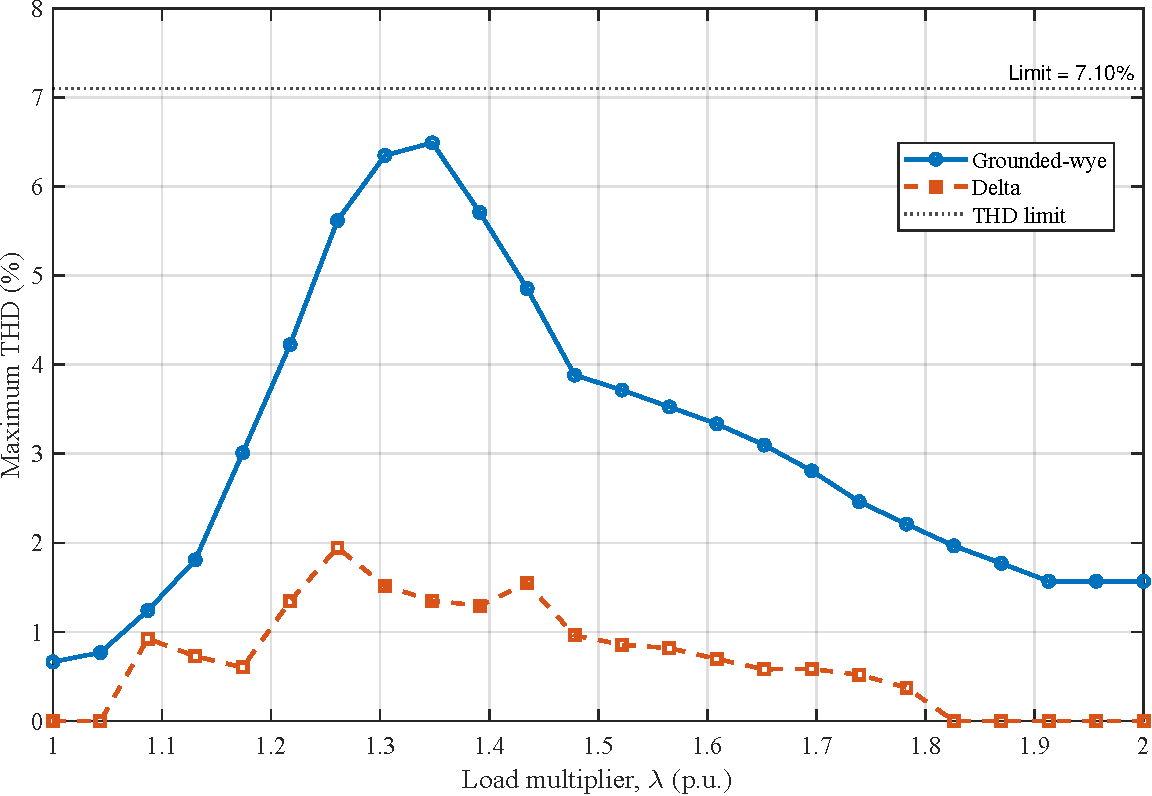
\includegraphics[width=\linewidth]{figuras_ieee123_equilibrado/maximum_THD_wye_delta.pdf}
    \end{minipage}\hfill
    \begin{minipage}[t]{0.49\textwidth}
        \centering
        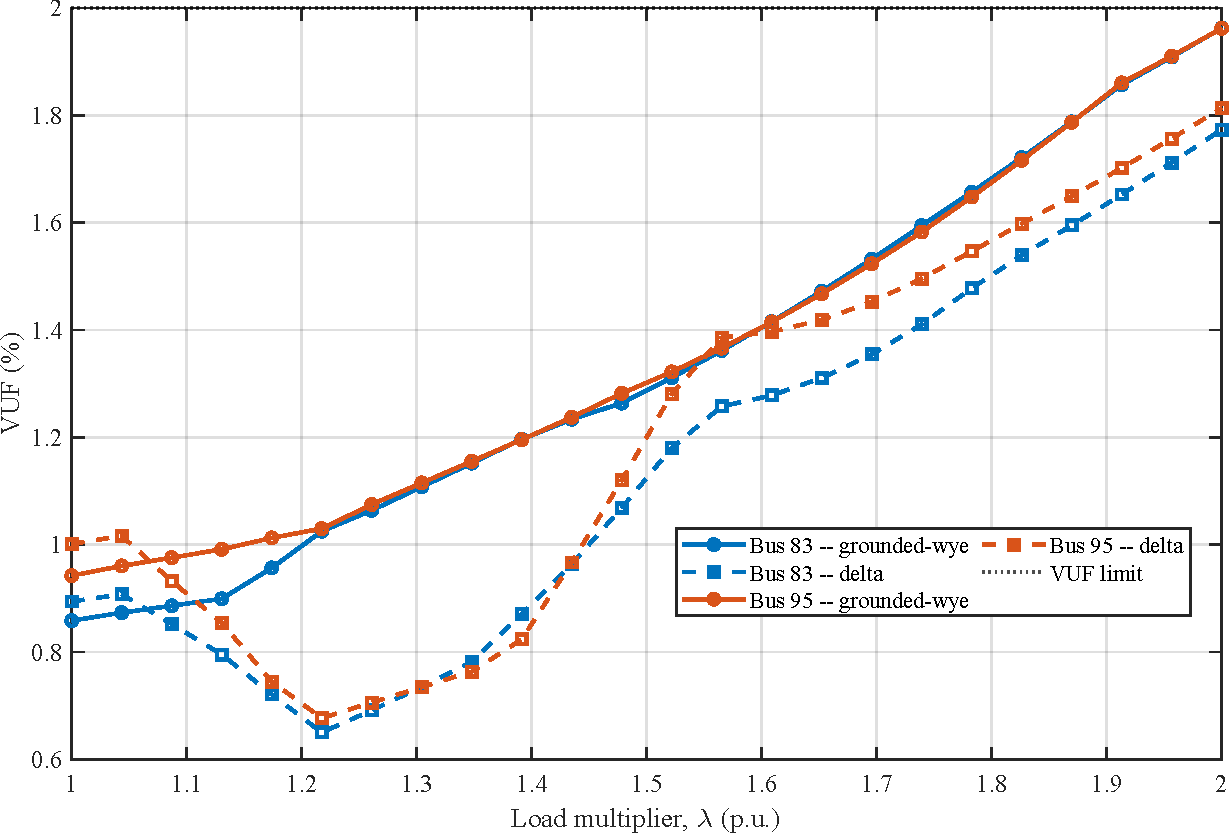
\includegraphics[width=\linewidth]{figuras_ieee123_equilibrado/VUF_controlled_buses_wye_delta.pdf}
    \end{minipage}
    \caption{Connection comparison over the balanced loading sweep: maximum
    feeder THD (left) and VUF at buses 83 and 95 (right). Solid curves denote
    grounded wye, and dashed curves denote delta.}
    \label{fig:ieee123_quality_connections}
\end{figure*}

The six controls are active over the sweep despite the equal phase
multipliers. For grounded wye at bus 83, the angle intervals for phases A, B,
and C are
$90.00^\circ$--$180.00^\circ$,
$90.00^\circ$--$116.43^\circ$, and
$90.00^\circ$--$178.96^\circ$, respectively. At bus 95, the corresponding
grounded-wye intervals are $90.00^\circ$--$180.00^\circ$,
$94.21^\circ$--$179.87^\circ$, and
$90.00^\circ$--$170.47^\circ$. The different phase trajectories are
consistent with the feeder's intrinsic unbalance and with independent
per-phase control; equal loading multipliers do not make the underlying
network electrically symmetrical. For delta, almost every $ab$, $bc$, and
$ca$ branch uses essentially the complete 90.00--180.00$^\circ$ interval.
The wider branch-angle excursions accompany the redistribution of compensation
through line-to-line elements and the cancellation of zero-sequence terminal
currents.

Fig.~\ref{fig:ieee123_angles_connections} shows how the grounded-wye phase
controls and delta branch controls change with loading. The trajectories also
explain the nonmonotonic THD curves: the harmonic response changes as individual
TCR elements move through different conduction regions and approach their
firing-angle bounds. The lower THD obtained with delta does not imply a lower
objective value because THD is imposed as a constraint rather than included
directly in~\eqref{eq:ieee123_balanced_objective}. The delta mean objective is
2.49, compared with 2.35 for grounded wye, reflecting its slightly weaker
high-loading voltage support despite the harmonic and VUF improvements.

\begin{figure*}[!t]
    \centering
    \begin{minipage}[t]{0.49\textwidth}
        \centering
        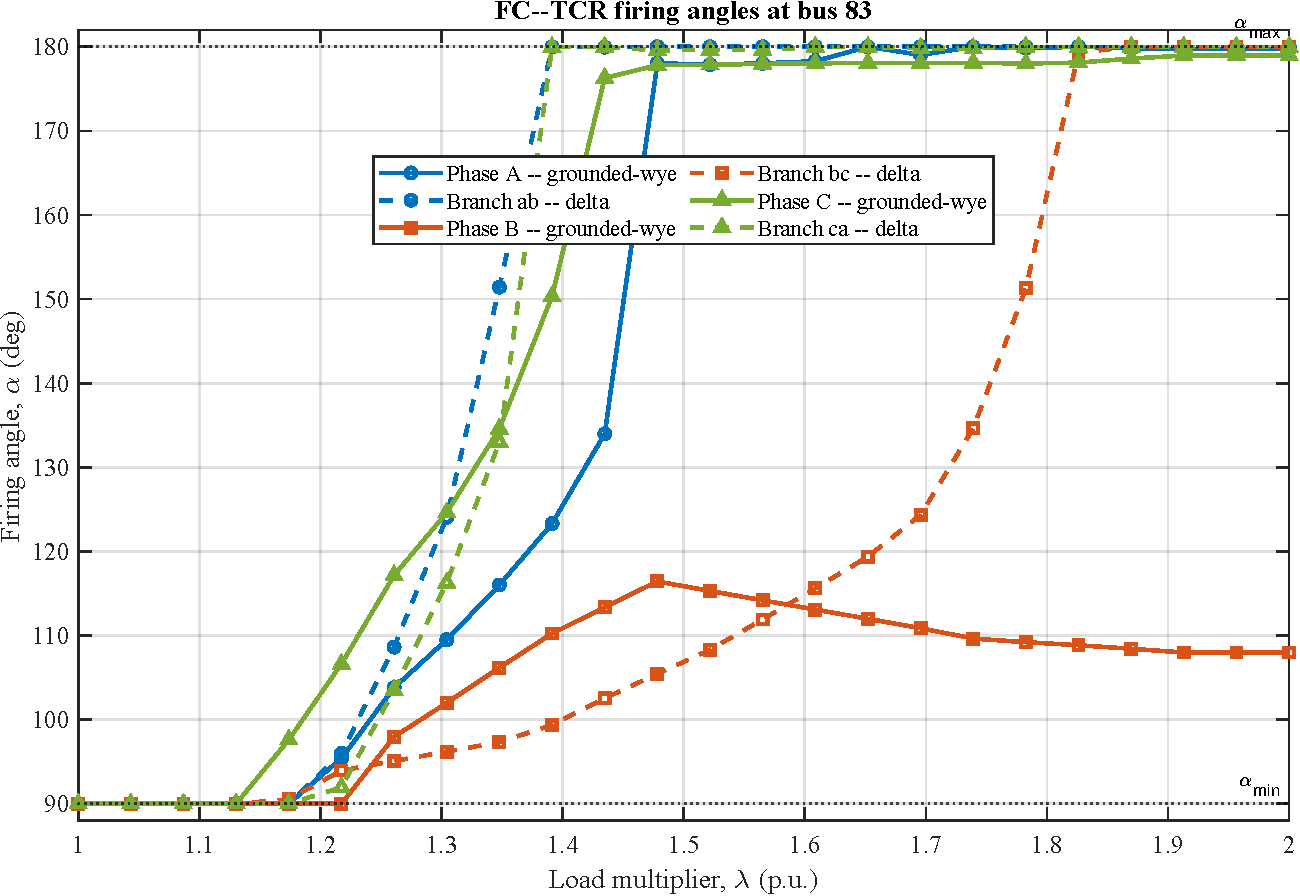
\includegraphics[width=\linewidth]{figuras_ieee123_equilibrado/firing_angles_bus_83_wye_delta.pdf}
    \end{minipage}\hfill
    \begin{minipage}[t]{0.49\textwidth}
        \centering
        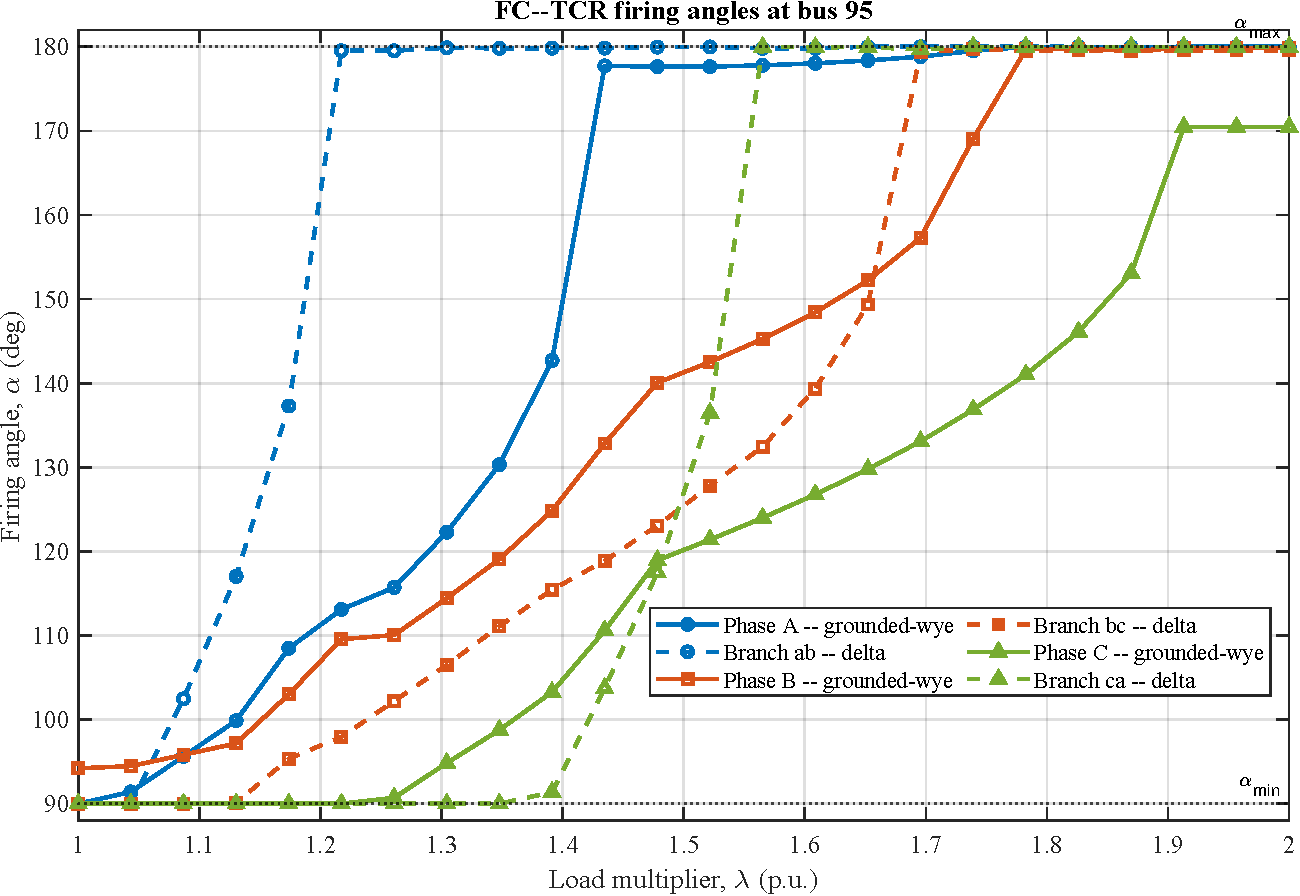
\includegraphics[width=\linewidth]{figuras_ieee123_equilibrado/firing_angles_bus_95_wye_delta.pdf}
    \end{minipage}
    \caption{FC--TCR firing angles at buses 83 (left) and 95 (right). Solid
    curves represent grounded-wye phase elements; dashed curves represent
    delta branches $ab$, $bc$, and $ca$.}
    \label{fig:ieee123_angles_connections}
\end{figure*}

\subsection{Computational time}

The computational performance of the proposed SQP-based approach was evaluated
for distribution systems with different sizes and operating conditions. The
tests comprise the 33-bus system under balanced and three-phase unbalanced
loading and the 123-bus system equipped with two grounded-wye SVCs, two delta
SVCs, and four grounded-wye SVCs. For the
balanced 33-bus case, the phase multiplier at each operating point was defined
as the mean of the three multipliers of the corresponding unbalanced case;
therefore, both curves preserve the same pointwise average loading. The
123-bus cases use the balanced-multiplier sweep from 1.00 to 2.00~pu.

The original SVCs of the 123-bus system are located at buses 83 and 95, and the
four-device case adds buses 72 and 300 according to the placement criterion
described at the beginning of Section~\ref{subsec:ieee123_results}.

All cases were executed sequentially in MATLAB R2024a on an Intel Core
i5-1135G7 processor with 19.8~GB of RAM. Table~\ref{tab:sqp_performance}
reports the arithmetic mean of the wall-clock time and the arithmetic mean of
the SQP iteration count over all 24 operating points of each curve. Thus, each
row represents the average computational cost of solving one operating point,
rather than the accumulated time of the complete loading trajectory or the
cost of an isolated worst case.

\begin{table}[!t]
\centering
\caption{Mean computational performance of the SQP approach over 24 operating points}
\label{tab:sqp_performance}
\footnotesize
\setlength{\tabcolsep}{3pt}
\renewcommand{\arraystretch}{1.1}
\begin{tabular}{@{}lcc@{}}
\toprule
System & Mean time (ms) & Mean iterations \\
\midrule
33-bus (balanced) & 7\,702.46 & 16.25 \\
33-bus (unbalanced) & 9\,399.73 & 17.33 \\
123-bus (two SVCs, grounded wye) & 10\,509.78 & 17.13 \\
123-bus (two SVCs, delta) & 7\,752.10 & 16.00 \\
123-bus (four SVCs, grounded wye) & 47\,998.79 & 44.08 \\
\bottomrule
\end{tabular}
\end{table}

The transition from the 33-bus to the 123-bus feeder increases the cost of each
reduced-space evaluation because the implicit state recovery must solve a much
larger global multifrequency HTPCIM system. Although the optimizer manipulates
only the SVC control variables, every evaluation of the objective function,
constraints, and derivatives still requires operations involving the complete
harmonic state and its Jacobian. For the same two-device arrangement, delta
requires 7\,752.10~ms per point on average, 26.24\% less than grounded wye,
while the mean iteration count decreases from 17.13 to 16.00. The two
connections have the same reduced dimension; therefore, this measured
difference is associated with the trajectories followed by the nonlinear
solver and optimizer, rather than with a smaller mathematical problem. All 24
electrically converged points are included in these means, independently of
their classification under the optimization inequalities.

Within the 123-bus feeder, adding two SVCs
doubles the reduced control dimension from six to twelve. This adds sensitivity
directions to the implicit linear solves, enlarges the constraint Jacobian and
the quadratic subproblem, and introduces additional coupling among the
compensators. The resulting search is also more demanding: the mean number of
SQP iterations increases from 17.13 to 44.08, so the greater cost of each
iteration is repeated substantially more often. Therefore, the approximately
4.57-fold increase in mean time is explained jointly by the greater work per
iteration and the larger number of iterations, rather than by the doubled
control dimension alone. Because the averages cover all 24 operating points
and include state solutions, sensitivity construction, quadratic-subproblem
solutions, and globalization steps, they represent the observed end-to-end
computational effort rather than a pure asymptotic complexity estimate.

\color{black}

\section{Conclusions}
\label{sec:conclusions}

This paper presented a reduced-space optimization approach for three-phase
SVC operation that combines voltage regulation, phase balancing, and harmonic
constraints while retaining the multifrequency network equations implicitly.
The 33-bus tests showed that independent branch controls reproduce symmetrical
operation under balanced loading and provide asymmetric compensation when the
phase demands differ.

The IEEE 123-node study extended the assessment to 3336 simultaneous states
and six controls associated with FC--TCR devices at buses 83 and 95. In the
balanced-multiplier sweep from 1.00 to 2.00~pu, all 24 grounded-wye cases and
all 24 delta cases converged electrically and were retained as valid operating
points. Grounded wye satisfied every optimization inequality at 22 points,
whereas delta did so at 21 points. The other converged points remain valid for
electrical analysis; their infeasible label indicates only that the imposed
0.95-pu minimum-voltage inequality was exceeded.

Delta substantially reduced the transfer of harmonic distortion to the feeder:
the mean pointwise maximum THD decreased from 3.09\% to 0.69\%, and the largest
THD decreased from 6.49\% to 1.95\%. It also reduced the largest VUF from
1.96\% to 1.81\%. Grounded wye, however, retained one additional
optimization-feasible loading point because its phase-to-ground branches
provided slightly stronger voltage support at high loading. The comparison
therefore exposes a connection-dependent tradeoff between harmonic and
unbalance mitigation and phase-to-ground voltage support. Future work should
investigate this tradeoff under additional harmonic orders, practical device
constraints, and other loading patterns.


\bibliographystyle{IEEEtran}
\bibliography{references}


\appendices
\section{System Data Used in the Simulations}
\label{app:system_data}

This appendix summarizes the active data set used to build the 33-bus test
system in the harmonic power-flow simulations. The notation is kept consistent
with the formulation adopted in the paper: $i$ denotes a bus, $\phi\in\Phi$
denotes a phase, $h$ denotes a harmonic order, and $j$ denotes an SVC bus. The
base quantities are $V_b=12.66$~kV, $S_b=1$~MVA, and
$Z_b=V_b^2/S_b=160.28~\Omega$. The fundamental frequency is 60~Hz, and the
harmonic set is $\mathcal{H}=\{1,3,5,7,11,13,15\}$. Bus 33 is the slack bus,
with balanced voltage magnitude 1.05~pu and phase angles $0.00^\circ$,
$-120.00^\circ$, and $120.00^\circ$.

The line parameters in \cite{dolatabadi2021} are the per-phase
series resistance and reactance before per-unit conversion. In the three-phase
model, the same self impedance is assigned to phases $a$, $b$, and $c$. The
mutual phase-coupling terms used in the data file are generated from the
corresponding self terms as one eighth of the self resistance and inductance,
and the shunt capacitance terms are derived from those mutual inductance
entries.



The phase-dependent load values used at each operating point are obtained from
Table~\ref{tab:appendix_load_data} according to
\eqref{eq:phase_load_scaling}. Entries written as a subtraction, such as
$90-200$, indicate that a fixed distributed-generation contribution is
subtracted from the local demand at that bus. In the uploaded data file, the
phase scaling coefficients are implemented through $A=1000\,d_a/S_b$,
$B=1000\,d_b/S_b$, and $C=1000\,d_c/S_b$, where $d_a$, $d_b$, and $d_c$ are
the phase loading multipliers. The ZIP composition is set as a constant-power
model.

\begin{table}[H]
\centering
\scriptsize
\caption{Nominal phase-load coefficients used in the ZIP load block}
\label{tab:appendix_load_data}
\setlength{\tabcolsep}{6pt}
\renewcommand{\arraystretch}{1.0}
\begin{tabular}{@{}ccc|ccc@{}}
\toprule
Bus & $P_i^0$ (kW) & $Q_i^0$ (kVAr) &
Bus & $P_i^0$ (kW) & $Q_i^0$ (kVAr) \\
\midrule
1  & 100 & 60  & 17 & 70 & 20 \\
2  & 90  & 40  & 18 & $90-200$ & 40 \\
3  & 120 & 80  & 19 & 90 & 40 \\
4  & 60  & 30  & 20 & 90 & 40 \\
5  & 60  & 20  & 21 & 90 & 40 \\
6  & 200 & 100 & 22 & $190-200$ & 50 \\
7  & 200 & 100 & 23 & 420 & 200 \\
8  & 60  & 20  & 24 & 420 & 200 \\
9  & 60  & 20  & 25 & $60-200$ & 25 \\
10 & 45  & 30  & 26 & 60 & 25 \\
11 & 400 & 350 & 27 & 60 & 20 \\
12 & 60  & 35  & 28 & 120 & 70 \\
13 & 120 & 80  & 29 & 200 & 600 \\
14 & 60  & 10  & 30 & 150 & 70 \\
15 & 60  & 20  & 31 & 210 & 100 \\
16 & 60  & 20  & 32 & $60-200$ & 40 \\
\bottomrule
\end{tabular}
\end{table}

\end{document}


